\documentclass[a4paper, 12pt]{article} % classe de base
\usepackage[utf8]{inputenc} % générer .bib avec zotero, encodage europe centrale 8859 2
\usepackage[american]{babel}	%
\usepackage{amsfonts,amssymb}
\usepackage{url}	
\usepackage{fancyhdr} 
\usepackage{multirow}
\usepackage{appendix}                                      
\usepackage{perpage}			
\usepackage[pdftex]{color,graphicx,graphics,epsfig}
\usepackage[square]{natbib} 
\usepackage{float}
\usepackage{amsmath} 
%\usepackage[hyper=true,toc=true,number=none,style=list]{glossary}
\usepackage[colorlinks=true]{hyperref} 
\hypersetup{urlcolor=blue,linkcolor=black,citecolor=red} 
\usepackage{setspace}
\usepackage{pdfpages}
\usepackage{listings}
\usepackage{xcolor}
\usepackage{subcaption}
\graphicspath{{figureLR/}{figure/}}
%for file in *.png; do convert $file -resize 800 ../figureLR/$file ; done
\setcounter{secnumdepth}{4}
\setcounter{tocdepth}{4}


\begin{document}
\renewcommand\bibname{Références bibliographiques}


\includepdf[pages=-]{Rw2_pages_Degarde.pdf} % page de titre fait dans word, plus maniable
\pagenumbering{arabic}
\newpage
 \section{Introduction}

Depuis 2017, l’Unité de Gestion des Ressources Forestières de l’Université de Liège (Gembloux Agro-Bio Tech), en partenariat avec l’IDF et le CNPF Grand-Est, participe au projet Regiowood-II, financé par le programme Interreg « Grand Région » englobant la Lorraine, la Wallonie, le Luxembourg et 3 länders allemands (Rhénanie Palatinat, Sarre et Bade-Wurtemberg. 
Ce projet s’axe autour de la reconstitution des forêts après coupes rases en s’appuyant notamment sur les données de la télédétection en contexte de crise sanitaire. (https://www.regiowood2.info/fr).\\
Dans le cadre de ce partenariat, il a été prévu que l’IDF, lors de son projet BioClimSol, développe un modèle de risque cartographié d’attaques de scolytes sur l’épicéa dans le Grand-Est et qu'une fois ce modèle développé, l’équipe de Gestion des Ressources Forestières de  Gembloux Agro-Bio Tech (Université de Liège), le teste en Wallonie et compare la démarche de BioClimSol à celle du Fichier Écologique.\\
Dans une première partie, ce rapport décrit les différentes étapes du processus d'adaptation du modèle de risques d’attaques de scolytes de BioClimSol en Wallonie.
Dans la seconde partie, il  teste le modèle BioClimSol et le compare avec la carte d'aptitude du fichier Écologique des essences.

La dernière partie compare l'intensité des attaques de scolytes entre les Vosges et la Wallonie selon des caractéristiques écologiques de sous-secteurs radiatifs et d'altitudes. Afin de détecter les attaques de scolytes, des cartes d'états sanitaires ont été réalisées à l'aide de l'imagerie satellite.

\newpage

 \section{Matériel et méthode}
 
 \subsection{Zone d'étude}
 
La zone d'étude de cette analyse est dans un premier la temps la Wallonie afin de réaliser une comparaison entre le modèle de risque BioClimSol et le Fichier Écologique des Essences. Les attaques de scolytes ont été détectées par imagerie satellitaire sur les tuiles T31UER, T31UES, T31UFQ, T31UFR, T31UFS, T31UGR des satellites Sentinel2 (voir figure \ref{tuiles}).



Dans un second temps, une tuile Sentinel 2 (T32ULU) couvrant une partie du massif des Vosges a été analysée avant de comparer des caractéristiques les attaques de scolyte entre la Wallonie et des Vosges.

%refaire figure moi meme elles sont pas très belles
\begin{figure} [htbp] 
    \centering
    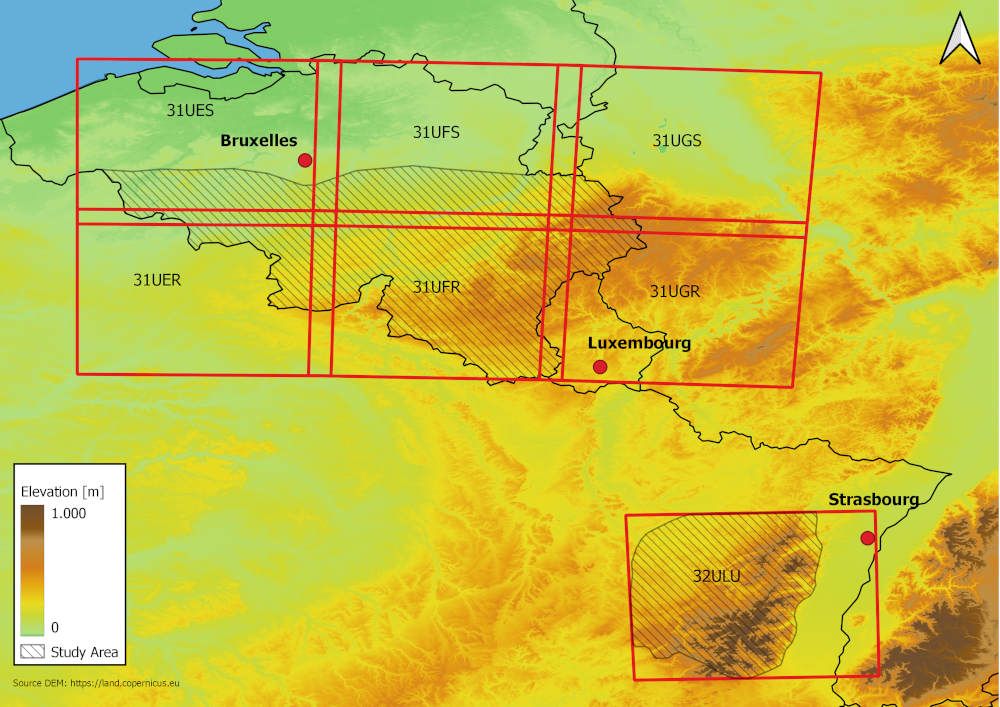
\includegraphics[width=1\textwidth]{waql_2.png}
    \caption{Zones d'étude de ce rapport}
    \label{tuiles}
\end{figure}
 

 \newpage
\subsection{Le modèle de risque d'attaque de scolyte de BioClimSol}
 
 \subsubsection{Introduction à BioClimSol.}
 BioClimSol est une méthode de diagnostic du peuplement
 intégrant le climat et ses extrêmes, et les conditions de terrain qui aggravent ou compensent le climat : sol, topographie, exposition.
Dans le cadre de ce projet, un modèle de risque d’attaques de scolytes (typographes et chalcographes) contre l’épicéa a été développé par l'équipe de l'IDF. \\


Ce modèle produit comme résultat une carte de risque sous la forme d'un indice de vigilance climatique (IBS). Cet indice reflète le niveau d'adéquation stationnelle de l'essence par rapport au risque d'attaque de scolytes. Il varie entre 0 et 10. Le niveau 0 exprime une absence de risque d'attaque de scolyte au cours d'une génération d'épicéa (0\%) alors que le niveau 10 exprime un risque d'attaque de 100 \% au cours d'une génération d'épicéa. Le niveau de risque acceptable est donc fixé par le propriétaire.
La section suivante décrit ce modèle, ainsi que les lignes de codes nécessaires pour produire une carte de risque d'attaque de scolytes en Wallonie.

\subsubsection{Variables et indices employés par le modèle épicéa de BioClimSol.}


Les tableaux \ref{tableabrute} et \ref{tableau_clim} récapitulent l'ensemble des variables écologiques nécessaires à la réalisation du modèle BioClimSol. L'ensemble des données climatiques a été fourni par l'IRM.


\begin{table}[htbp]
\caption{Tableau récapitulatif des indices topographiques}
\label{tableabrute}
\begin{tabular}{|l|l|l|l|l|}
\hline
\textbf{Variable tographique}              & \textbf{Abreviation} & \textbf{Unité} & \textbf{Valeurs} & \textbf{Résolution}   \\ \hline
MNT                          & MNT                  & m              & [ 0 ; 690.9 ]        & 50 m    \\ \hline
Pente                        & pente\_p             & \%             & [0 ; 135.45]       & 50 m     \\ \hline
Pente                        & pente\_rad           & rad            & [0 ; 1.29]        & 50 m   \\ \hline
Exposition                   & aspect\_p            & \%             & [0 ; 360]         & 50 m    \\ \hline
Exposition                   & Aspect\_r            & rad            & [0 ; 6.28]        & 50 m   \\ \hline
Topographic   position index & tpi                  &                & [-22.16 ; 22.63]   & 50 m    \\ \hline
Saga Wetness   Index         & SWI                  &                & [4.17 ; 15.80]     & 50 m    \\ \hline
Visible Sky                  & vs                   &                & [70 ; 100]          & 50 m   \\ \hline
IKR de Becker                & ikdb                 &                & [-1.01 ; 1.42]     & 50 m    \\ \hline


\end{tabular}
\end{table}
 
 \begin{table}[htbp]
 
\caption{Tableau récapitulatif des indices climatiques}
\label{tableau_clim}

\begin{tabular}{|l|l|l|l|l|}
\hline
\textbf{Indice climatique}                                                                                                                                                                                                      & \textbf{Abreviation} & \textbf{Unité} & \textbf{Valeurs} & \textbf{Résolution} \\ \hline
\begin{tabular}[c]{@{}l@{}}Somme de la différence \\ des précipitations  mensuelles \\et de l'évapotranspiration \\ mensuelles de Turc \\entre le 1er mai et\\ 30 septembre pour la moyenne\\  trentenaire.\end{tabular} & PETP30               & mm             & [134.10 ; 157.10]   & 5km                 \\ \hline
\begin{tabular}[c]{@{}l@{}}Somme de la différence\\ des précipitations \\ et de l'évapotranspiration\\ de Turc mensuelle\\ entre le 1er mai et \\ le  30 septembre pour 2018.\end{tabular}                                 & PETP2018             & mm             & [-464.21 ; 600.40]  & 5km                 \\ \hline
Degrés Jour                                                                                                                                                                                                          & DJ                   & °C             & [-557 ; 1284.9]      & 5km                 \\ \hline
\begin{tabular}[c]{@{}l@{}}Température maximum du jour\\ le plus chaud \\ entre mai et septembre\end{tabular}                                                                                                           & XTX 2018             & °C             & [31.9 ; 38.09]       & 5km                 \\ \hline
\end{tabular}
\end{table}
\newpage
\subsubsection{Équations du modèle de risque BioClimSol pour l'épicéa}

Le modèle BioClimSol emploie deux sous modèles: un modèle climatique et un modèle topographique. Le modèle climatique (\ref{eq:Eq_mode_clim}) est ensuite inséré dans le modèle topographique (\ref{eq:Eq_mode_topo}). 

\paragraph{Équation modèle climatique}


\begin{equation}\label{eq:Eq_mode_clim}
Logit_{clim} = a - (b* PETP_{30}) -(c*PETP_{2018})+ (d*XTX_{2018}) + (e* DJ)
\end{equation}
  
\begin{itemize}

\item a = -14.3
\item b = 0.00557 
\item c = 0.00608
\item d = 0.265
\item e = 0.00212

\end{itemize}  
\paragraph{Équation modèle topographique}
 
\begin{equation}\label{eq:Eq_mode_topo}
Logit_{TOPO} = a - (b* PENTE_{p}) -(c*TPI)+ (d*IKDB) + (e* VS) + (f*SWI) + (g*LC)
\end{equation}    
\begin{itemize}

\item a =  - 12.9 
\item b = 0.0302 
\item c = 0.035
\item d =  0.230
\item e =  0.111
\item f = 0.224
\item g = 0.443

\end{itemize}
\subsubsection{Code sous R de calculs des variables et indices}

Le modèle BioClimSol emploie deux types de variables, variables topographiques et variables climatiques.
Les variables topographiques sont issues du MNT et sont calculées à l’aide des logiciels Saga Gis, Orfeo ToolBox et GDAL.
Pour la Wallonie, les variables climatiques ont été fournies par l’Institut Royal Météorologique (tableau \ref{tableau_clim}).
Les variables topographiques employées, leurs unités, leurs formats ainsi qu’un ordre de grandeurs sont mentionnés dans le tableau \ref{tableabrute}.

\paragraph{Variables climatiques}

\subparagraph{Estimation de l’ETP de Turc }

Comme données initiales, l’Institut Royal Météorologique (IRM) nous a fourni l’ETP de Penman. Or le modèle BioClimSol emploie l’ETP de Turc. L’ETP de Turc a été calculée à l’aide d’une régression linéaire. Cette régression linéaire a été réalisée à l’aide d’un jeu de données reprenant des valeurs mensuelles d’ETP de Turc et de Penman de toute la France pour l’année 2018. \\ 

\textbf{ETP\textunderscore Turc} = \textit{ -7.498+ 0.949 x ETP\textunderscore Penman }

%%%%%%%


\subparagraph{somme des degrés jours (DJ) }


somme au 30 septembre d’une année donnée des
températures moyennes journalières excédant 8.3°C et 557 °C au total de la somme.
\\
$\sum_{}^{1/01 \mapsto 30/09}  DJ_{base 8.3} - 587$




\subparagraph{Estimation des températures maximales entre mai et septembre (XTX2018)}
Pour obtenir la température maximale entre mai et septembre, la température maximum du jour le plus chaud par pixel de 5km X 5km a été conservée dans ce raster.




\paragraph{Variables topographiques.}




\subparagraph{	Pente (\%) et exposition (radian) } 

Fonction : [SAGA] Slope, aspect, curvature \\
Input : MNT [m] \\
Note : Les valeurs de pente et d'exposition sont exprimées en pourcentage et degrés pour l’affichage cartographique, et en radians pour les besoins du calcul \\

\textbf{Ligne de commande employée:} \\
\begin{quote}
\texttt{ta\textunderscore morphometry 0 -- ELEVATION  [MNT]  -- SLOPE[pente\textunderscore pourcent.sdat] \; --ASPECT [exposition.sdat] \; -- METHOD \; 6\; --UNIT\textunderscore SLOPE \; 0  -- UNIT\textunderscore ASPECT \;0 }
\end{quote}

\subparagraph{TPI -Topographic Position Index} 

Fonction : [SAGA] Topographic position index (tpi) \newline
Input : Altitude [m]\\
\textbf{Ligne de commande employée:} 
\begin{quote}
\texttt{ta\textunderscore morphometry \textit{18} -- \textit{DEM [mnt]} --TPI [tpi\textunderscore 150.sdat] -- \textit{STANDARD 0} --RADIUS\textunderscore MIN 0 --RADIUS\textunderscore MAX 100 --DW\textunderscore WEIGHTING 0 --DW\textunderscore IDW\textunderscore POWER 1 --DW\textunderscore IDW\textunderscore OFFSET 1 --DW\textunderscore BANDWIDTH 75}
\end{quote}
\subparagraph{Visible sky} 

Fonctions : [SAGA] Sky view factor Input : Altitude [m]. Note : Le VS est calculé dans un rayon de 2000 m. \\
\textbf{Ligne de commande employée:} 
\begin{quote}
\texttt{ ta\textunderscore lighting 3 --DEM [MNT] --VISIBLE [vs.sdat] --SVF [svf.sdat] --RADIUS 2000 --METHOD              0 --DLEVEL 3 --NDIRS 8}
\end{quote}
\subparagraph{SWI} 

Fonction : [SAGA] Saga wetness index \\
Input : Altitude [m] \\
\textbf{Ligne de commande employée:} 
\begin{quote}
 \texttt{ ta\textunderscore hydrology 15 --DEM [MNT] --AREA [area\textunderscore mod.sdat] --SLOPE [slope\textunderscore mod.sdat] --AREA\textunderscore MOD [out\textunderscore 3] --TWI [swi.sdat] \; --SUCTION 10 \; --AREA\textunderscore TYPE 0 \; --SLOPE\textunderscore TYPE 0 --SLOPE\textunderscore MIN 0 \; --SLOPE\textunderscore OFF 0.10 --SLOPE\textunderscore WEIGHT 1}
\end{quote}

\subparagraph{IKR de Becker – Indice de climat lumineux de Becker }


L’indice de climat lumineux défini par Becker exprime l’énergie lumineuse reçue sur une station, en pourcentage de l’énergie reçue par un plan de référence de même surface mais parfaitement horizontal. Il se calcule par la formule suivante : 
\begin{align*}
IKR=\frac{\sin(C-\arctan((pente)*\cos(exposition)))}{\sin(C)}
\end{align*}

avec C étant une constante calculée ci-dessous sur base de la latitude et peut se calculer avec l'équation :

\begin{equation}

$C = -0.0146* latitude + 1.5192$ 

\end{equation}

Ci-dessous se trouve les différentes étapes afin de calculer cet indice:
\begin{enumerate}
   

        \item  \textbf{Calcul latitude}\\
Fonction : [GRASS] r.latlong \\
Note : reporter l’emprise du raster en input  dans l’entrée Emprise de la région GRASS GIS 7 (xmin, xmax, ymin,ymax)\\
\textbf{Ligne de commande employée:} 
\begin{quote}
\texttt{ r.latlong --l [pente\textunderscore radian.sdat] output=[latitude.sdat]}
\end{quote}
 
 

        \item \textbf {Calcul constante C}
\begin{quote}
 \texttt{otbcli\textunderscore BandMath --il [latitude.sdat] --out [constante\textunderscore C.tif] \; uint8 \; --exp " -0.0146\times im1b1 + 1.5192 "} 
   \end{quote}
  
        \item \textbf {Calcul de l’IKR de Becker} \\


\textbf{Ligne de commande employée:}
\begin{quote}
 \texttt{otbcli\textunderscore BandMath --il l[altitude.sdat] [pente\textunderscore rad.tif]
 [exposition\textunderscore rad.tif] --out [IKR.tif] --exp  " \sin(im1b1-\atan(im2b1\times \cos(im3b1)))/ \sin(im1b1) " } \\
   
   \end{quote}

\end{enumerate}

\subsection{Le fichier Écologique des essences }


Le fichier Écologique des Essences est une boite à outils comprenant des cartes de caractéristiques stationnelles (niveau trophique, hydrique et zones bioclimatiques) et des fiches essences synthétisant l'autécologie des principales essences forestières de Wallonie.

Les figures \ref{fig:nt} et \ref{fig:nh} représentent les clefs de détermination permettant de réaliser respectivement les cartes de niveau trophique et hydrique à partir de varibales écologiques abiotiques, cartographiques ou récoltées sur le terrain.

Le niveau trophique est une caractéristique stationnelle estimé à partir du pH,de la lithologie et du développement de profil du sol tandis que le niveau hydrique est déterminé sur base de la profondeur, de la texture et  de l'hydromorphie du sol ainsi que  de l'apport en eau.
%mettre grille 

\begin{figure} [htbp] 
    \centering
    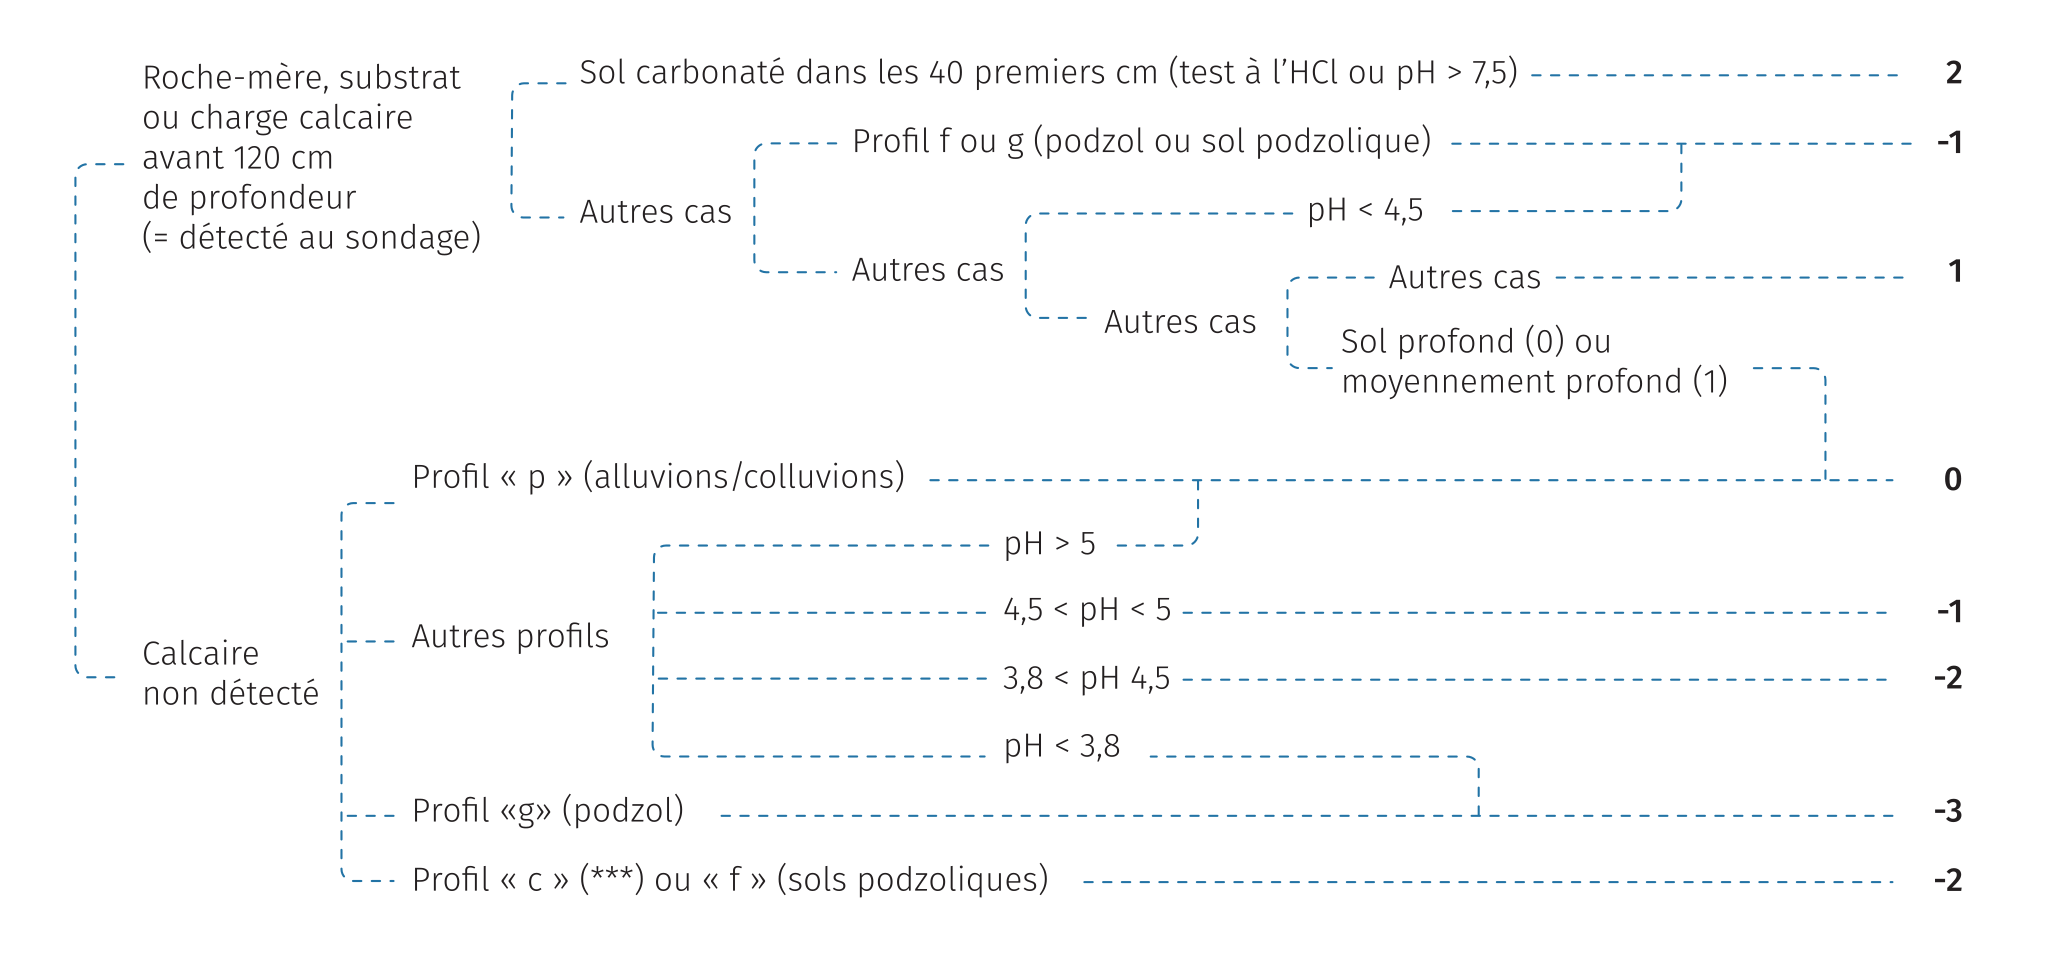
\includegraphics[width=0.8\textwidth]{nt.png}
    \caption{Clef de détermination du niveau trophique (fichierecologique.be)}
    \label{fig:nt}
\end{figure}
 
\begin{figure} [htbp] 
    \centering
    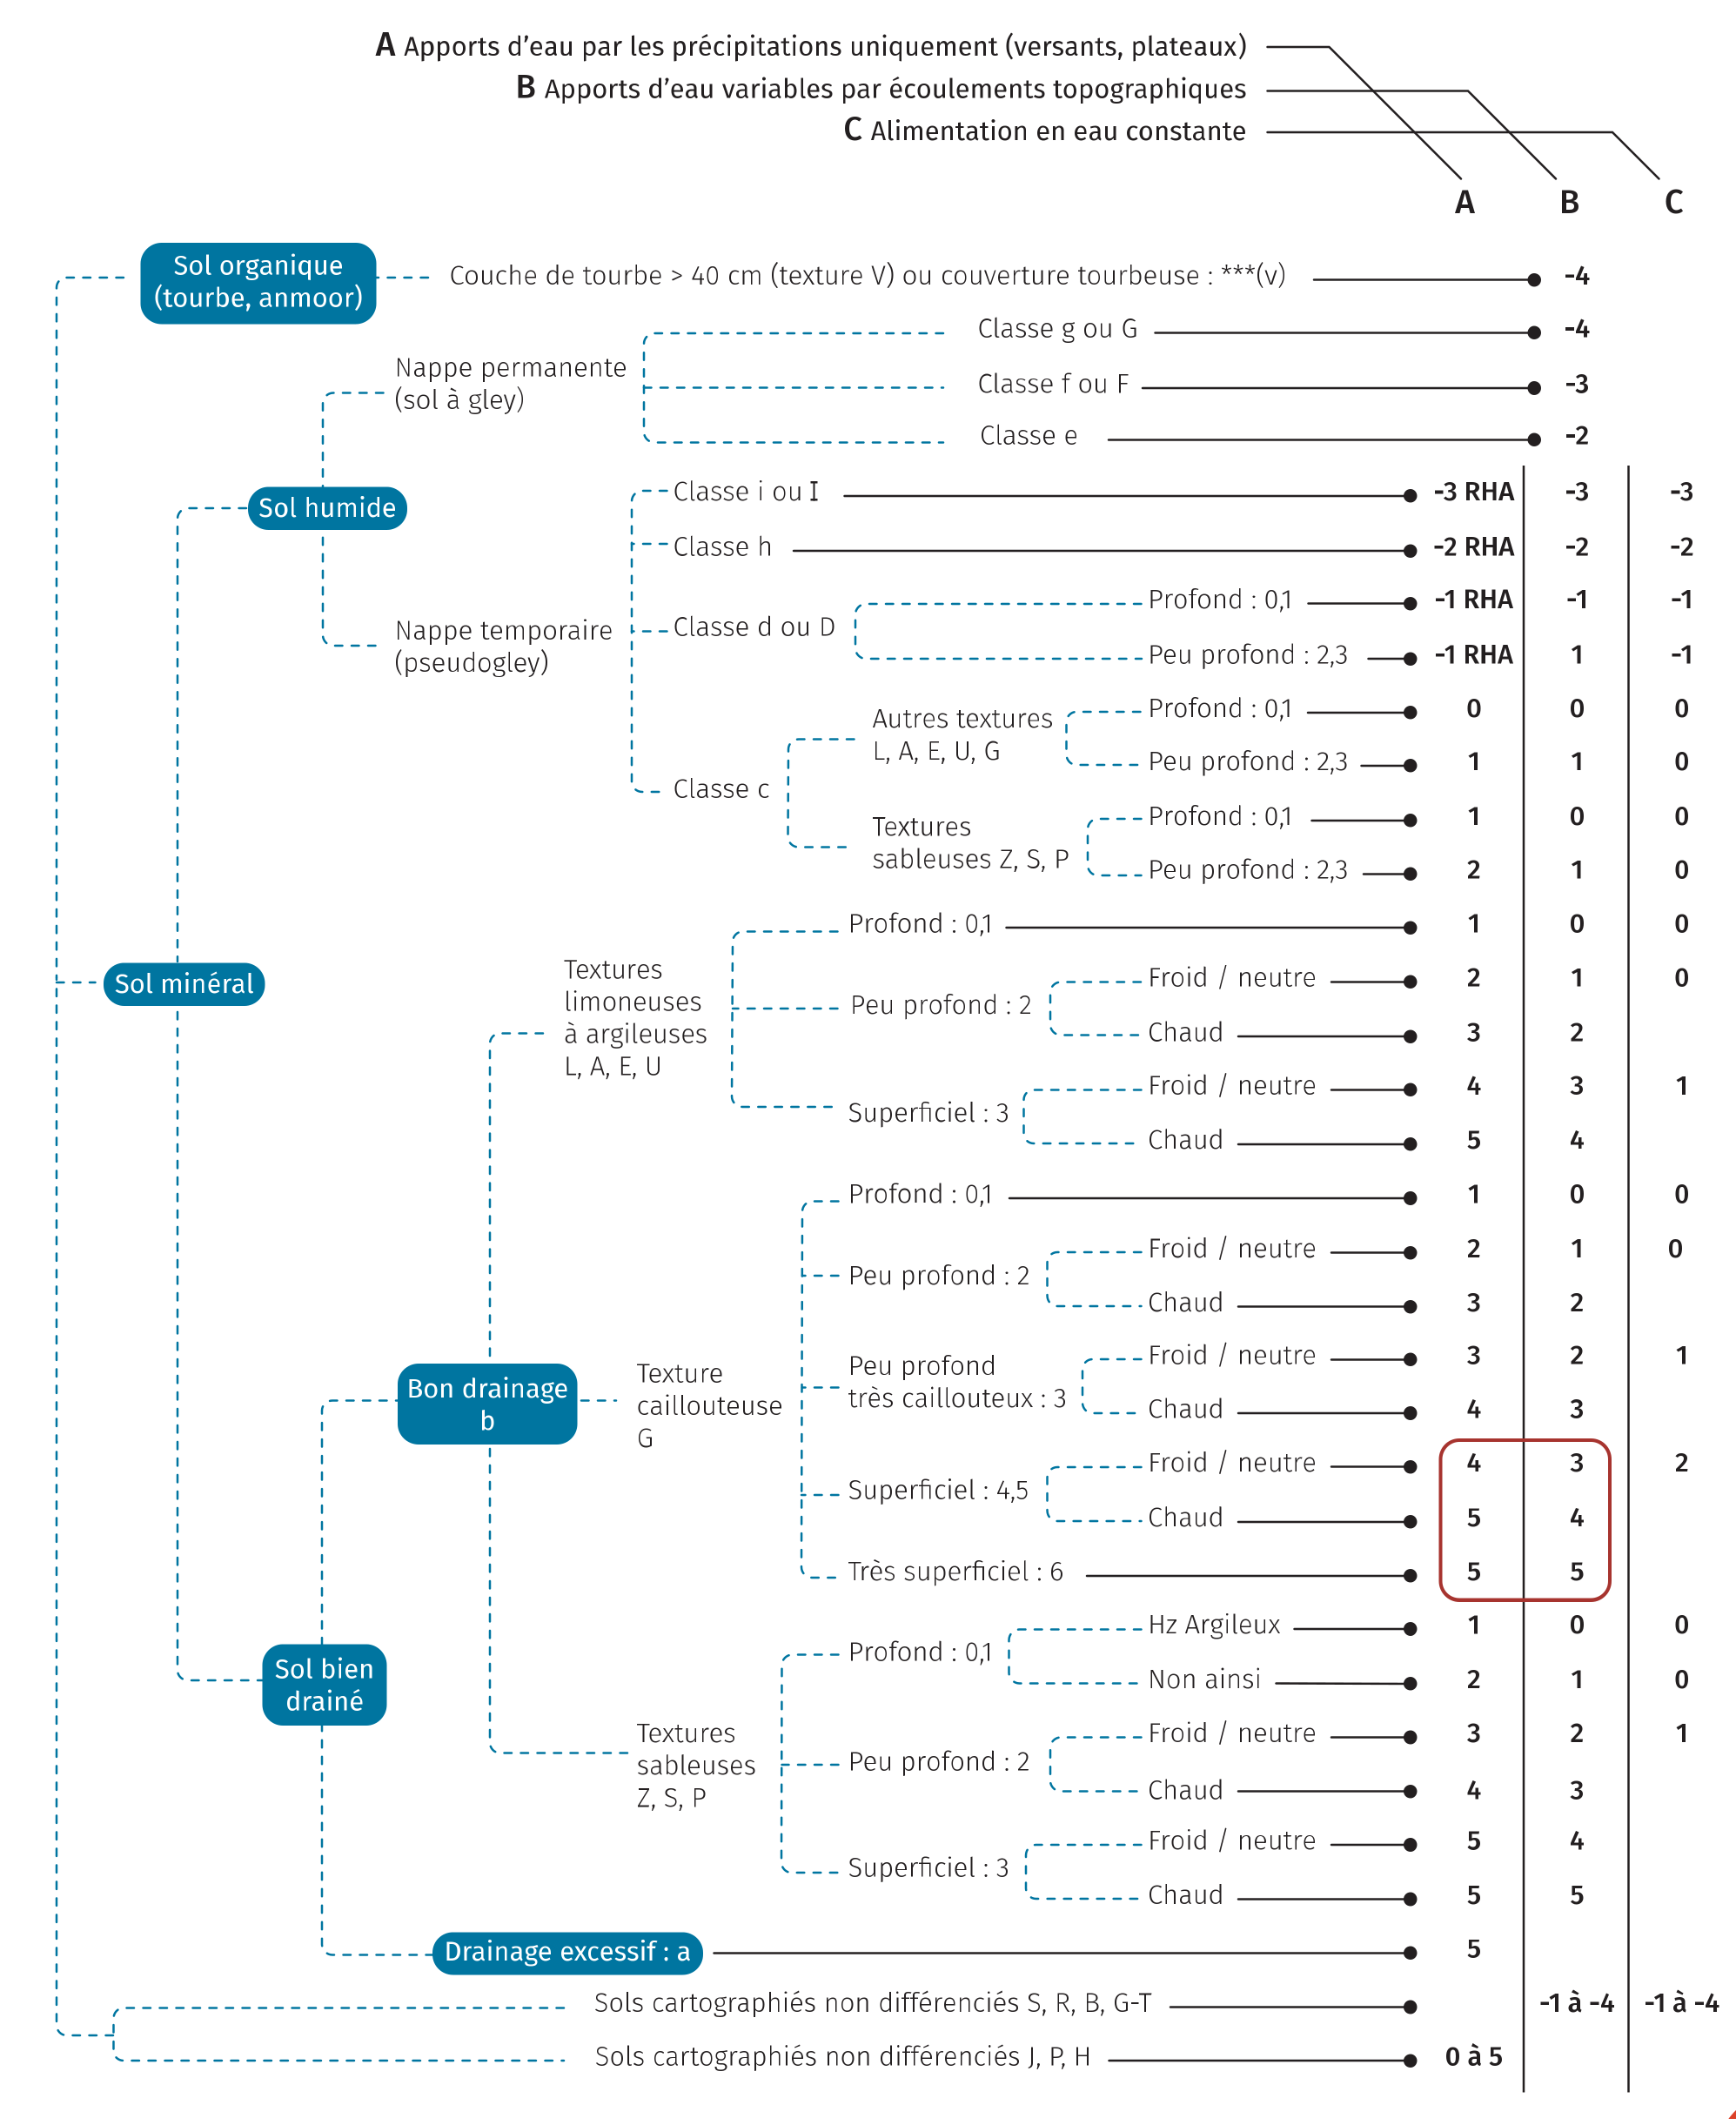
\includegraphics[width=0.9 \textwidth]{nh.PNG}
    \caption{Clef de détermination du niveau hydrique (fichierecologique.be) }
    \label{fig:nh}
\end{figure}


L'écogramme de la fiche essence de l'épicéa commun est présente sur la figure \ref{fig:eco}.
\begin{figure} [htbp] 
    \centering
    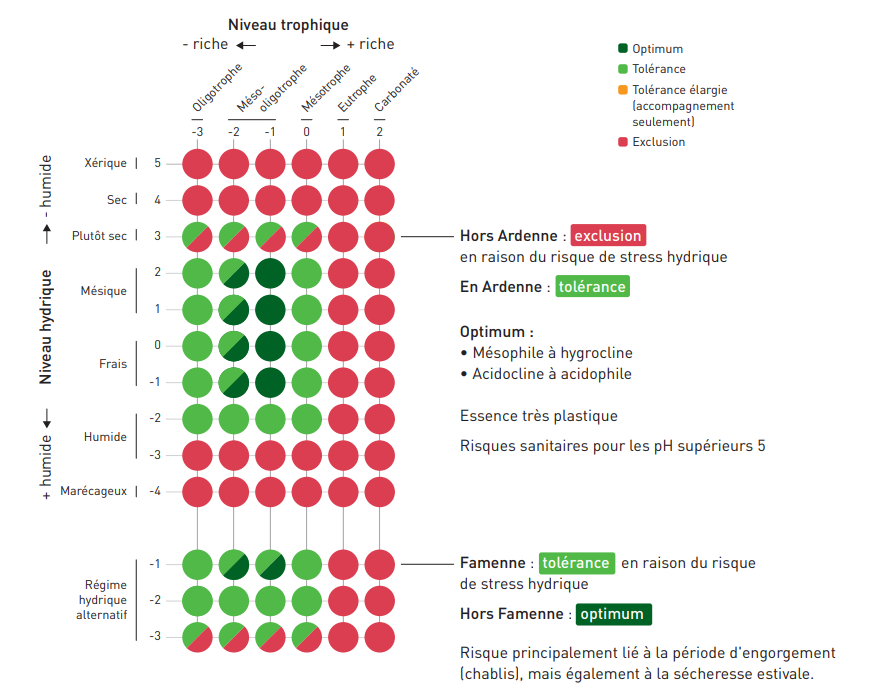
\includegraphics[width=0.9 \textwidth]{eco.PNG}
    \caption{Ecogramme d'aptitude de l'épicéa (fichierecologique.be). Le cas d'incertitude entre tolérance et optimum pour le niveau trophique -2 ne peut être levé que par une analyse chimique du sol. }
    \label{fig:eco}
\end{figure}

La carte de sensibilité climatique de l'épicéa est présente sur la figure \ref{fig:sens}.
\begin{figure} [htbp] 
    \centering
    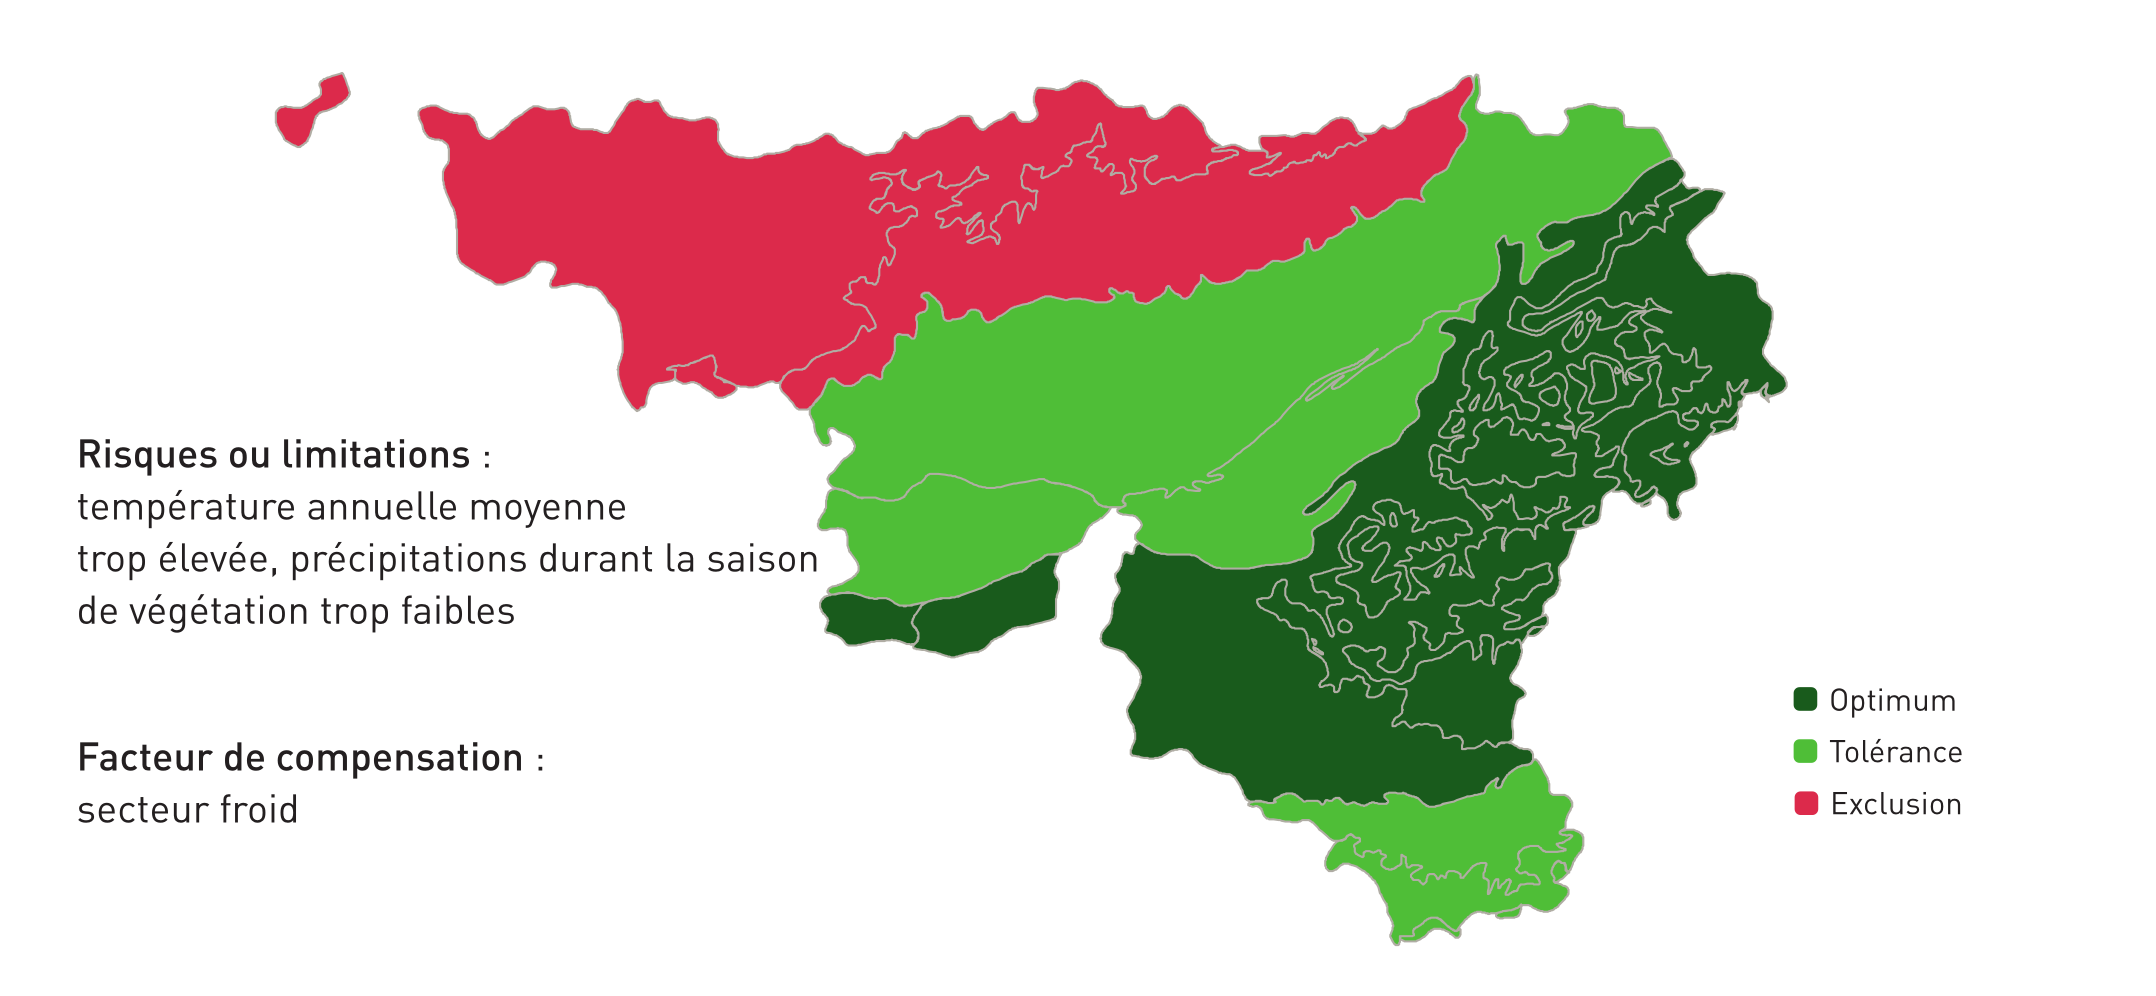
\includegraphics[width=0.9\textwidth]{sensibilite_ep.png}
    \caption{Carte de sensibilité climatique de l'épicéa en Wallonie à l'échelle du macroclimat des zones biogéoraphiques (fichierecologique.be).}
    \label{fig:sens}
\end{figure}
Les différentes zones bioclimatiques de la Wallonie sont indiquées sur la figure \ref{fig:zbio}.
\begin{figure} [htbp] 
    \centering
    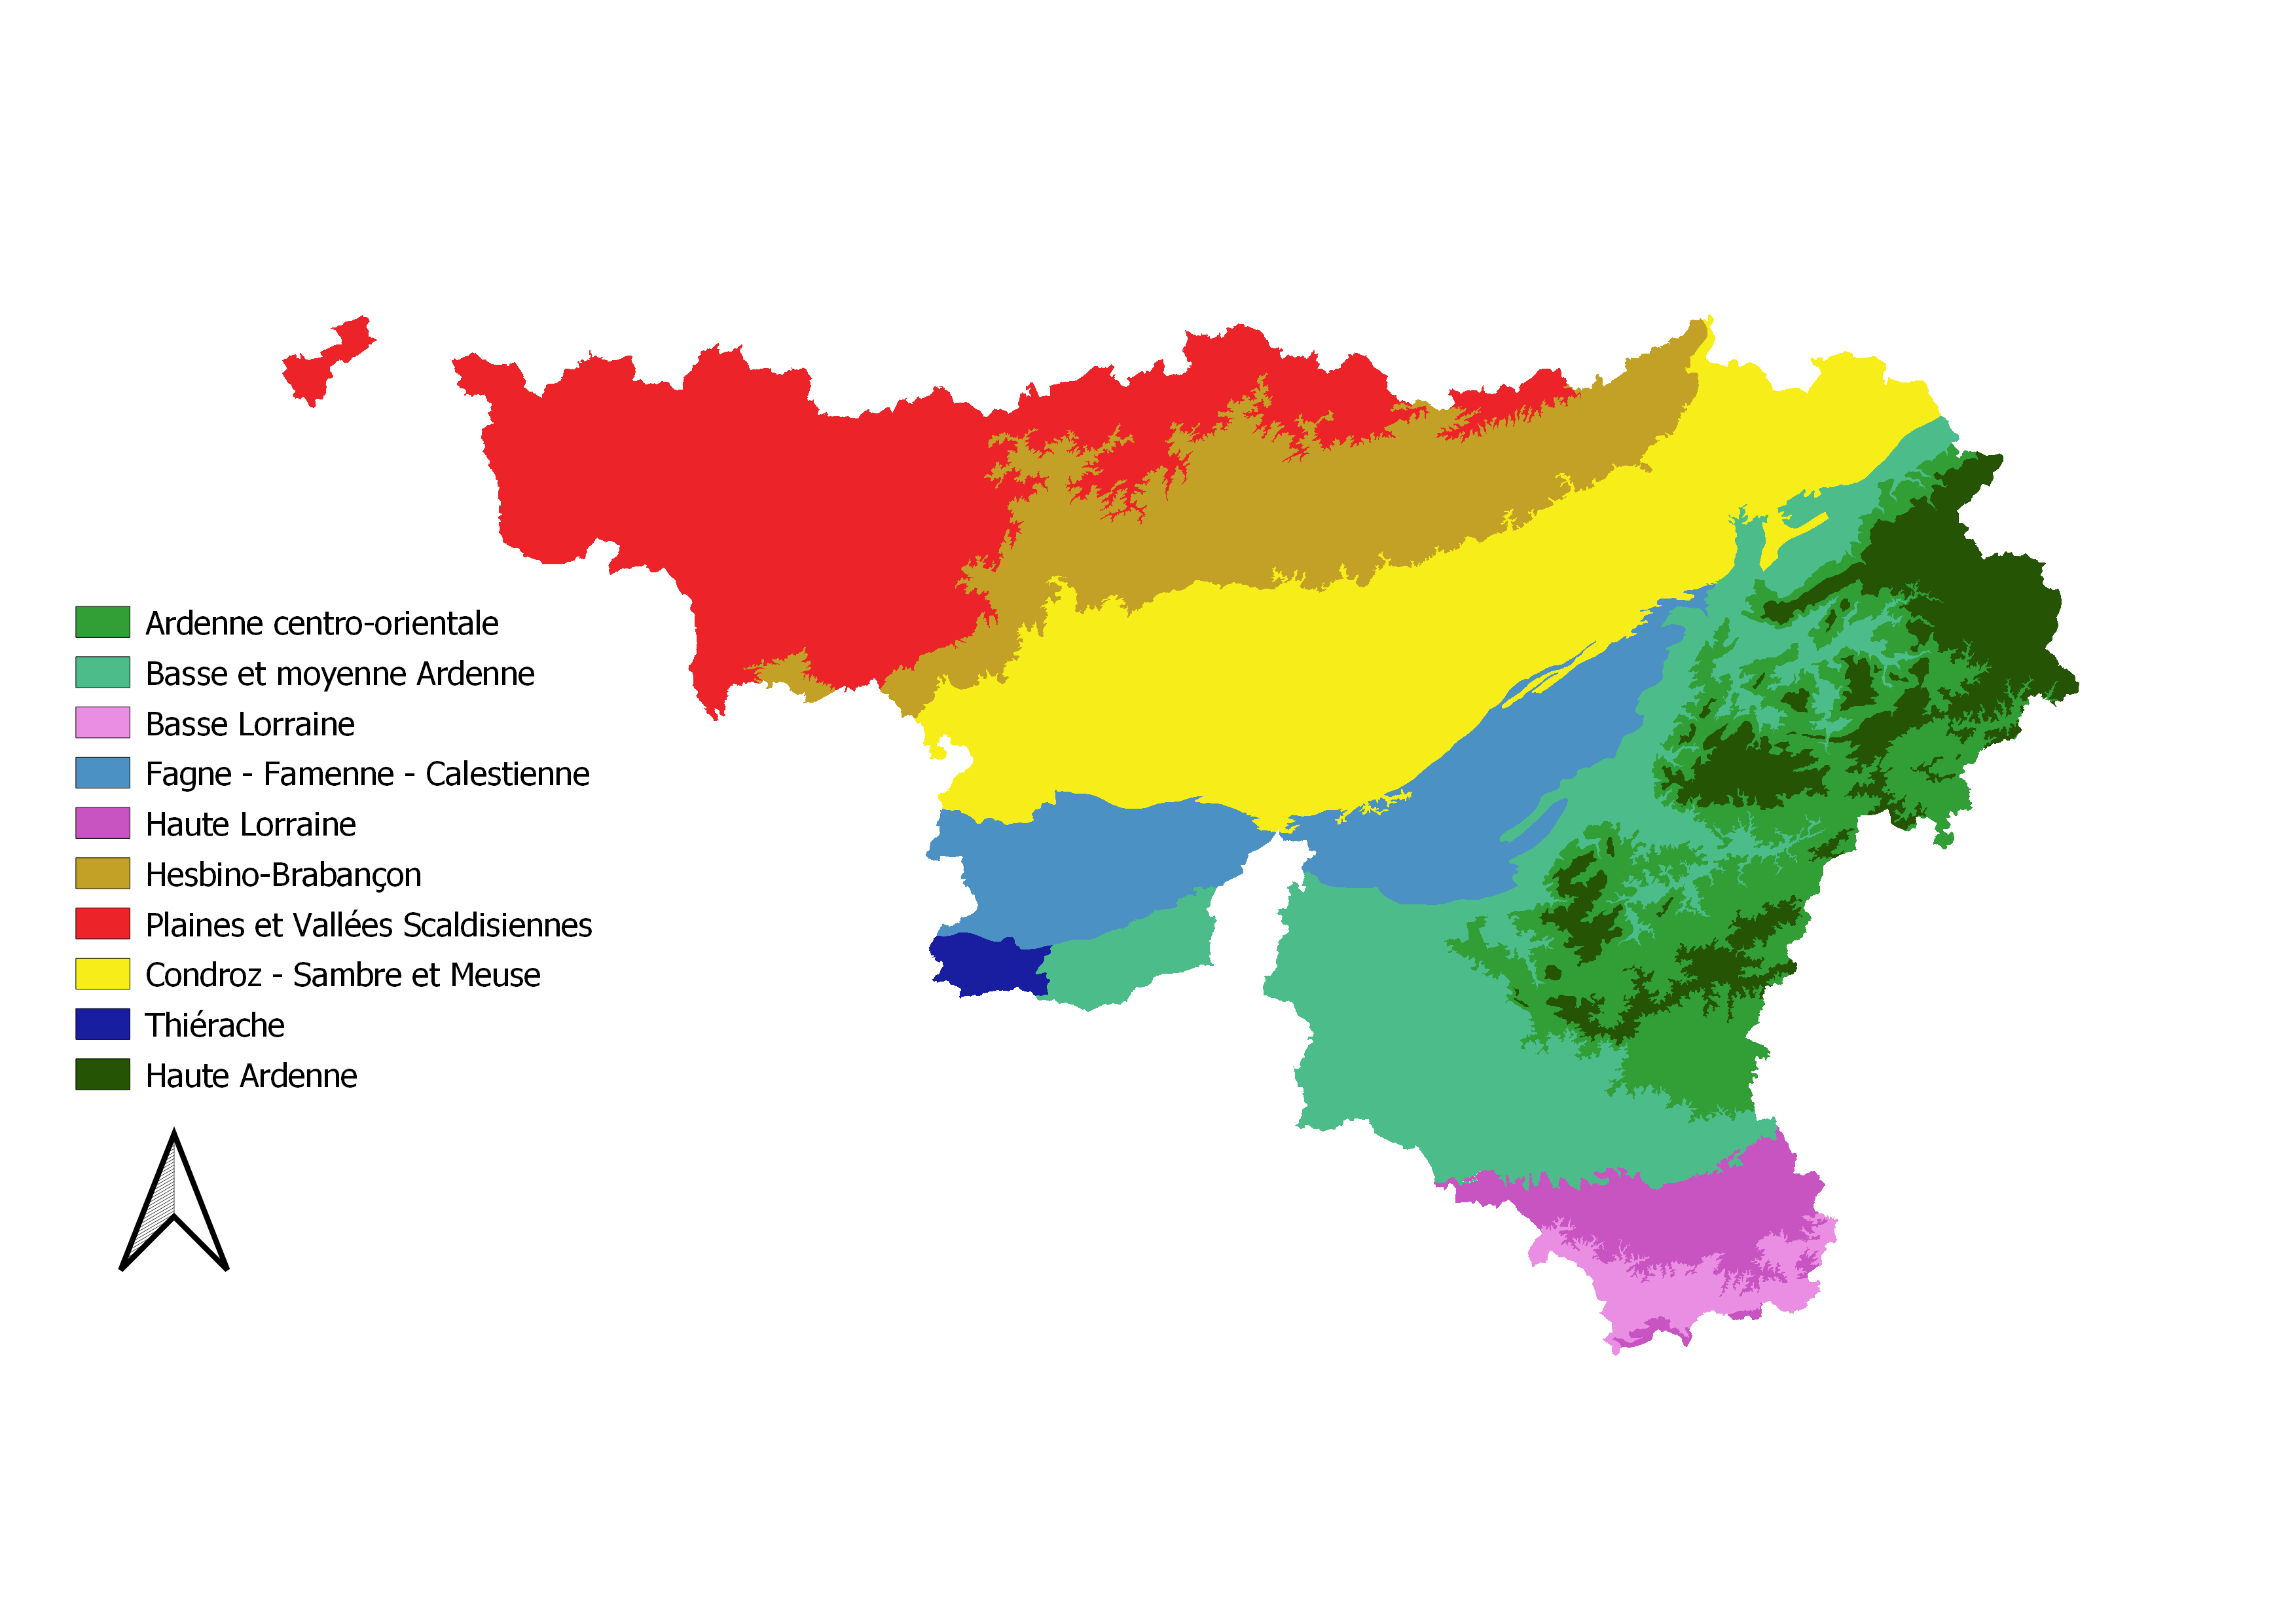
\includegraphics[width=0.9\textwidth]{zbio.png}
    \caption{Carte des zones bioclimatique de la Wallonie \citep{van_der_perre_carte_2015}.}
    \label{fig:zbio}
\end{figure}


Les cartes créés sur base des figures  \ref{fig:nt}, \ref{fig:nh} et \ref{fig:eco} sont ensuite croisées pour obtenir la carte d'aptitude de l'essence pour la Wallonie. 
Les différents niveaux d'aptitude de cette carte pour l'épicéa commun sont:

\begin{enumerate}
    \item OPTIMUM: Optimum écologique et sylvicole de l'essence. Elle peut être utilisé sans limite sur la station.
    \item TOLÉRANCE: Bon développement de l'essence bien que certains facteurs limitant affectent la stabilité ou la productivité de l'essence.
    \item EXCLUSION: Impossibilité de développement de l'essence à long terme sur la station 
\end{enumerate}

\newpage
\subsection{Confrontation des cartes de risque BioClimSol et d'aptitude du Fichier Ecologique des Essences avec les estimations de dégâts de scolytes.}
Afin d'estimer les dégâts causés par les scolytes de l'épicéa (typographe et chalcographes), des cartes d'états sanitaires de la pessière Wallonne ont été réalisées sur base de la méthodologie de l'INRAe \citep{dutrieux_mise_2021,dutrieux_package_2021}. Ces cartes ont été développées grâce aux images sentinel 2 à l'aide d'un indice spectral.
L'indice spectral employé pour la détection des épicéas dépérissant (à partir du stade vert) est le CRSWIR:
\begin{align*} 
CR_{SWRIR} &= \dfrac{SWIR1}{( NIRa + (\lambda_{SWIR1}-\lambda_{NIRa})* (\dfrac{SWIR2 - NIRa}{\lambda_{SWIR2}-\lambda_{NIRa}})} \\ 
avec&\\ 
\lambda_{NIRa} &=865\\ 
\lambda_{SWIR1} &=1610\\ 
\lambda_{SWIR2} &=2190
%\end{equation*}
\end{align*} 

%bofbof
L'ensemble de la méthodologie de calcul des cartes d'états sanitaires est présente dans \cite{lisein_guide_2022}.

Afin d'estimer les dégâts aux pessières de Wallonie et des Vosges, les probabilités de présence de scolyte  ont été calculées sur base des cartes d'état sanitaire annuelles et de une ou  plusieurs cartes de caractéristiques écologiques (altitude, sous-secteurs radiatif ou les deux en même temps).

Cette probabilité est le ratio de la surface scolytée d'une classe d'une carte de caractéristiques écologiques sur la surface totale qu'occupe la même classe de la carte de caractéristiques écologiques.
L'équation suivante est un exemple de calcul de la probabilité de présence de scolyte pour la classe d'altitude 100-200m en Wallonie.
%mettre env
%%%%corrr

\begin{figure} [htbp] 
    \centering
    
\includegraphics[width=0.8\textwidth]{CodeCogsEqn .png}
   
    \label{fig:eq}
\end{figure}
\nexpage
\section{Résultats}

\subsection{Cartes de risque BioClimSol et d'aptitude Fichier Écologique des Essences.}
Le résultat obtenu pour le modèle BioClimSol est un raster de l'indice de vigilance BioClimSol variant 0 à 10 (figure \ref{fig:fin}). Le 0 indique un faible risque d’attaque de scolyte et le 10 un risque élevé d’attaque.


On considère qu'une essence est à exclure de la station à partir d'un niveau 5. Pour les nouvelles plantations, un niveau 0 ou 1 est vivement recommandé.  
Dans le cas où le niveau de risque tolérable est de maximum 1, l’épicéa pourrait survivre dans les vallées pentues et dans l’est dans la Wallonie. L'est de la Haute-Ardenne serait la région où le risque d'attaque de scolytes serait le plus faible.

D'après ce modèle, planter de l'épicéa dans les régions bioclimatiques au nord sillon Sambre et Meuse (Plaines et vallées Scaldisiennes et Hesbino-Brabançon) est très risqué, excepté dans certaines vallées.

\begin{figure} [htbp] 
	\centering
	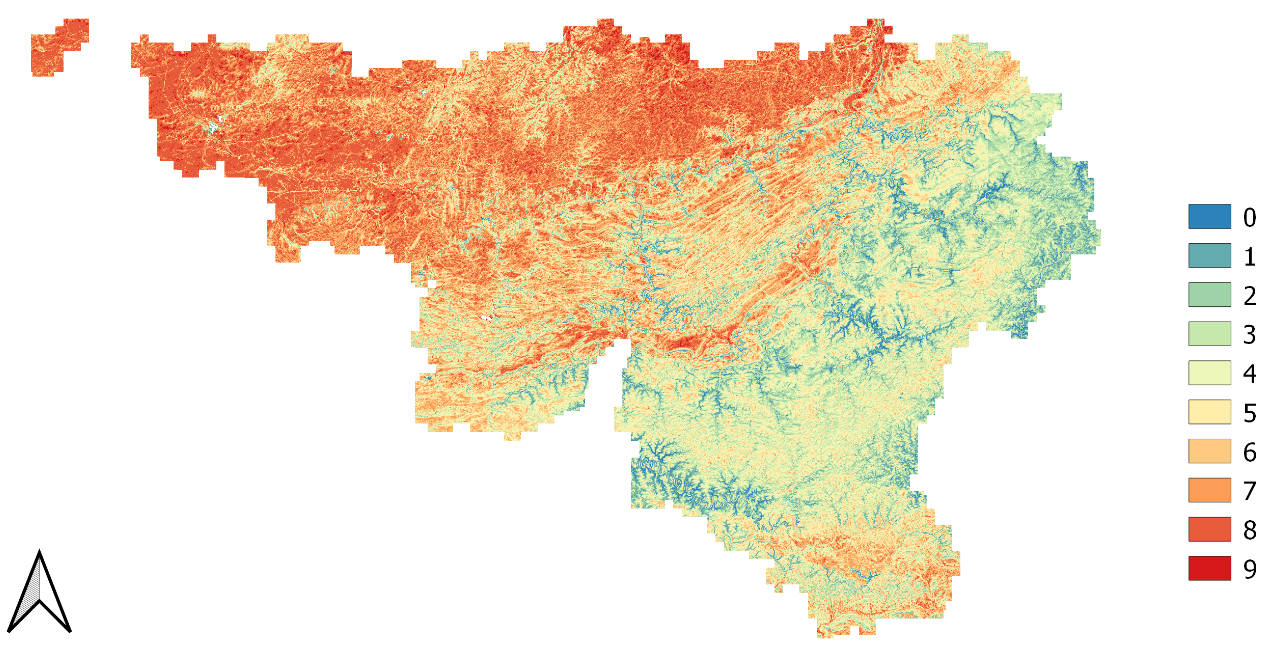
\includegraphics[width=1\textwidth]{fin.png}
	\caption{Carte de résultats du modèle de risque d'attaque de scolytes BioClimSol}
	\label{fig:fin}
\end{figure}


A l'échelle régionale, la carte d'aptitude du Fichier Écologique des Essences montre que l'épicéa est en exclusion dans tout le nord du sillon Sambre et Meuse ainsi qu'en Calestienne (sud de la Famenne). Elle l'indique globalement l'épicéa en tolérance dans les régions Bioclimatiques Sambre-et-Meuse et Condroz et Basse et Haute Lorraine.
Par ailleurs, l'épicéa est en optimum sur une grande partie de la Basse et moyenne Ardenne, sur l'Ardenne centro-orientale et la haute Ardenne, à l'exception de la zone de tourbières et sols à argiles blanches des Hautes Fagnes (Nord-Est)


\begin{figure} [htbp] 
	\centering
	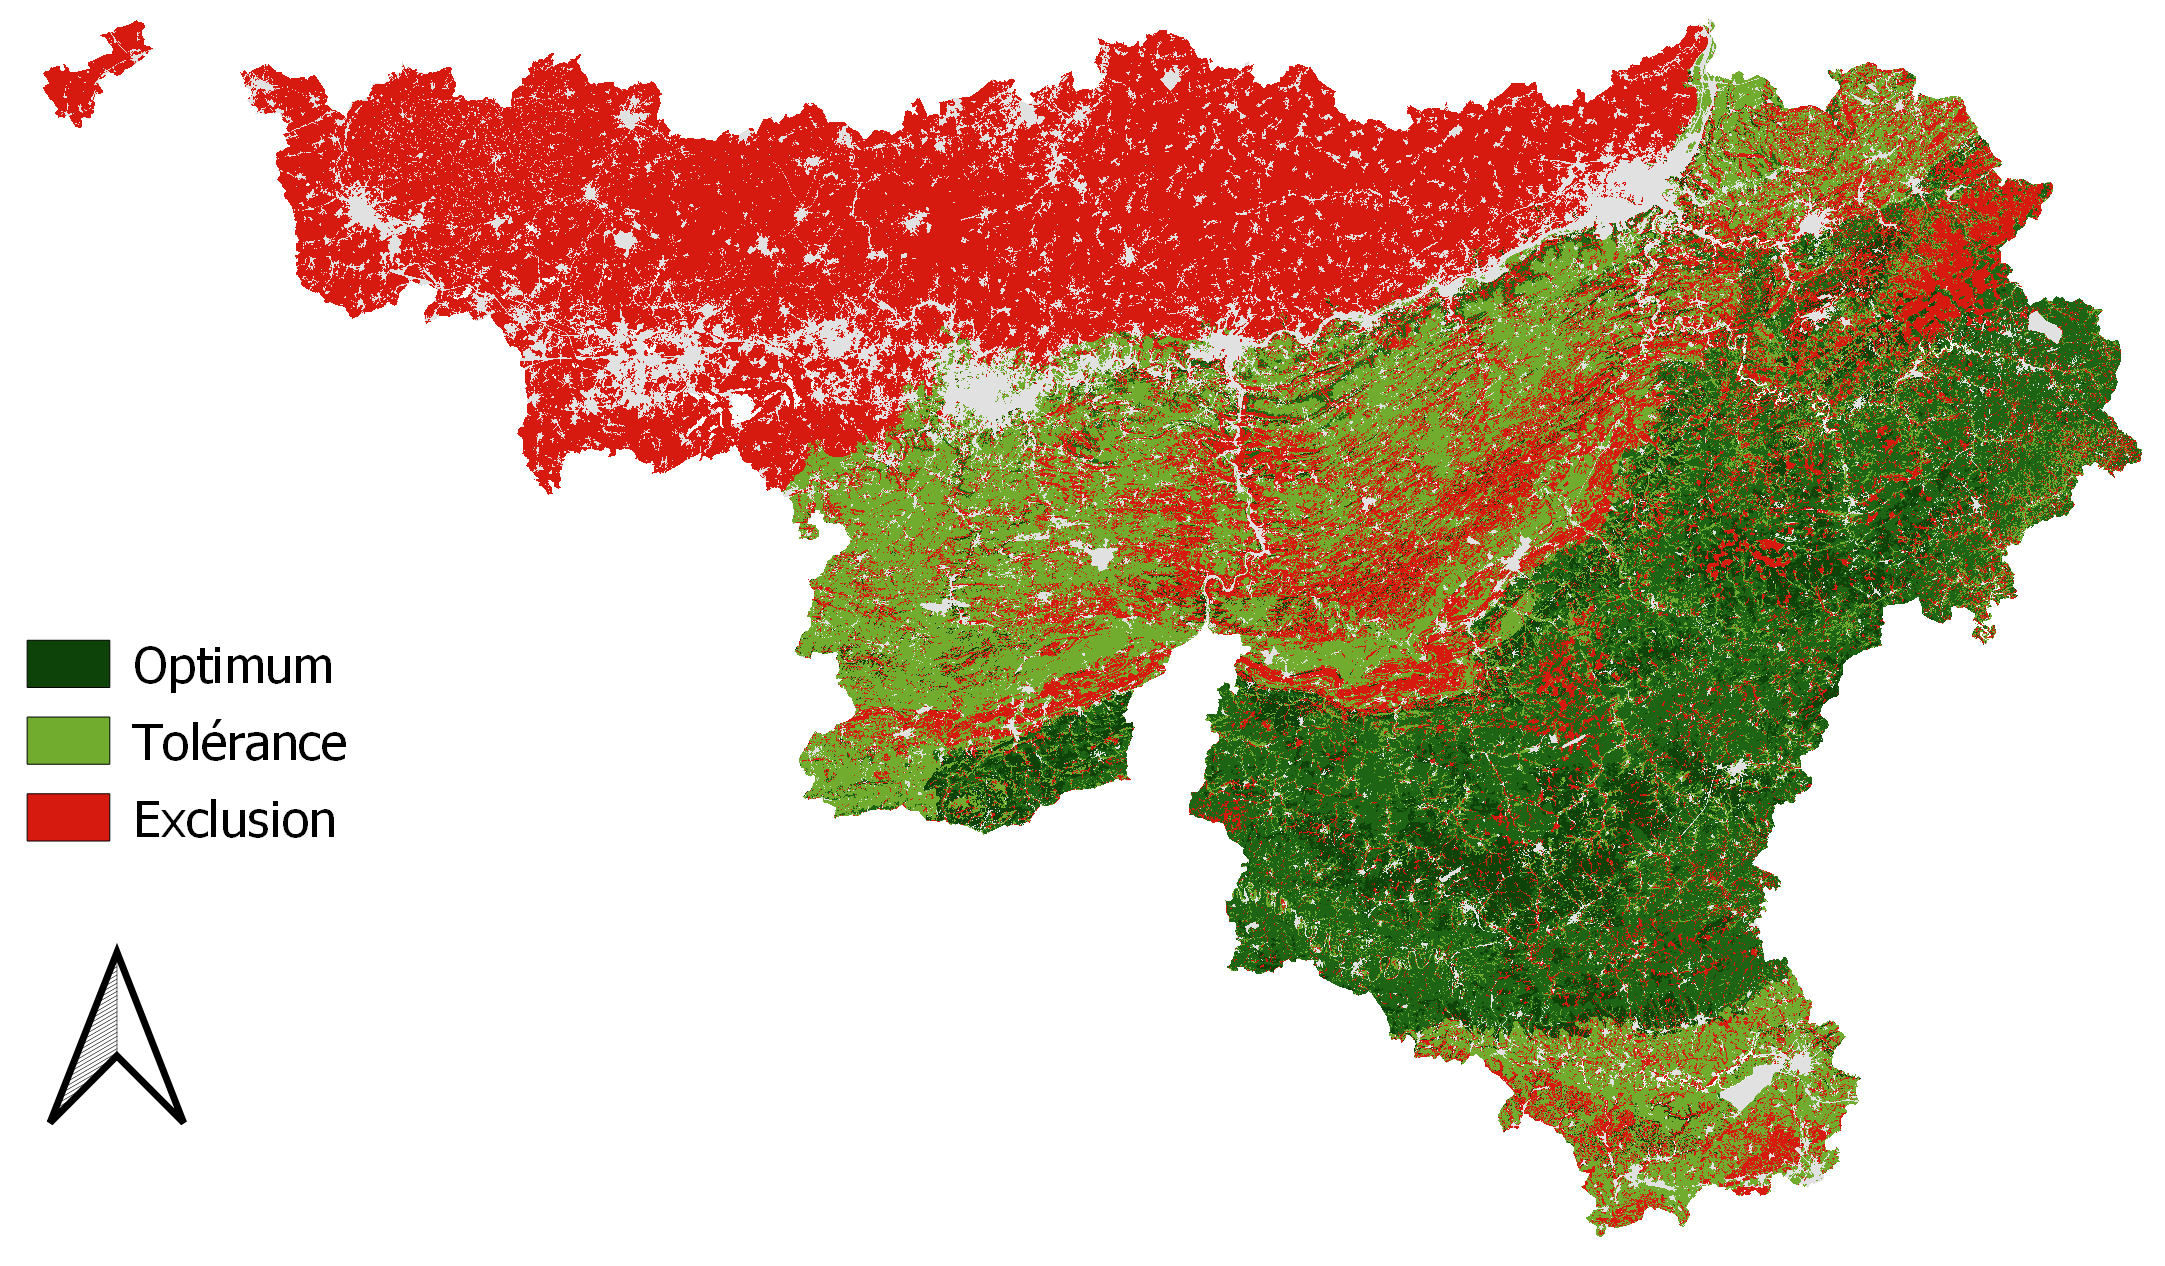
\includegraphics[width=1\textwidth]{ep.png}
	\caption{Carte d'aptitude du Fichier Écologique des Essences.La teinte verte intermédiaire est une indétermination de l’aptitude
		(entre tolérance et optimum) qui ne peut être levée que par une analyse chimique du sol }
	\label{fig:feev}
\end{figure}






La carte d'aptitude du Fichier Écologique de Essences (Figure \ref{fig: la_roche_1}) indique l'épicéa  en optimum (ou presque) sur la majorité des plateaux, à l'exception des grandes zones d'exclusion qui correspondent en réalité à des sols très hydromorphes voire tourbeux. Sur les versants, l'épicéa est considéré en tolérance dans les versants sud et en optimum sur les orientations nord.
La carte de risque de BioClimSol (Figure \ref{fig: la_roche_2}) indique quant à elle un faible risque dans les versants (0 à 1), quelque soit leur orientation, mais une risque élevé sur tous les plateaux (5 à 7) et dans la plaine alluviale (N-W de la carte).








\begin{figure}[htbp]
	\begin{minipage}[b]{1 \linewidth}
		\centering
		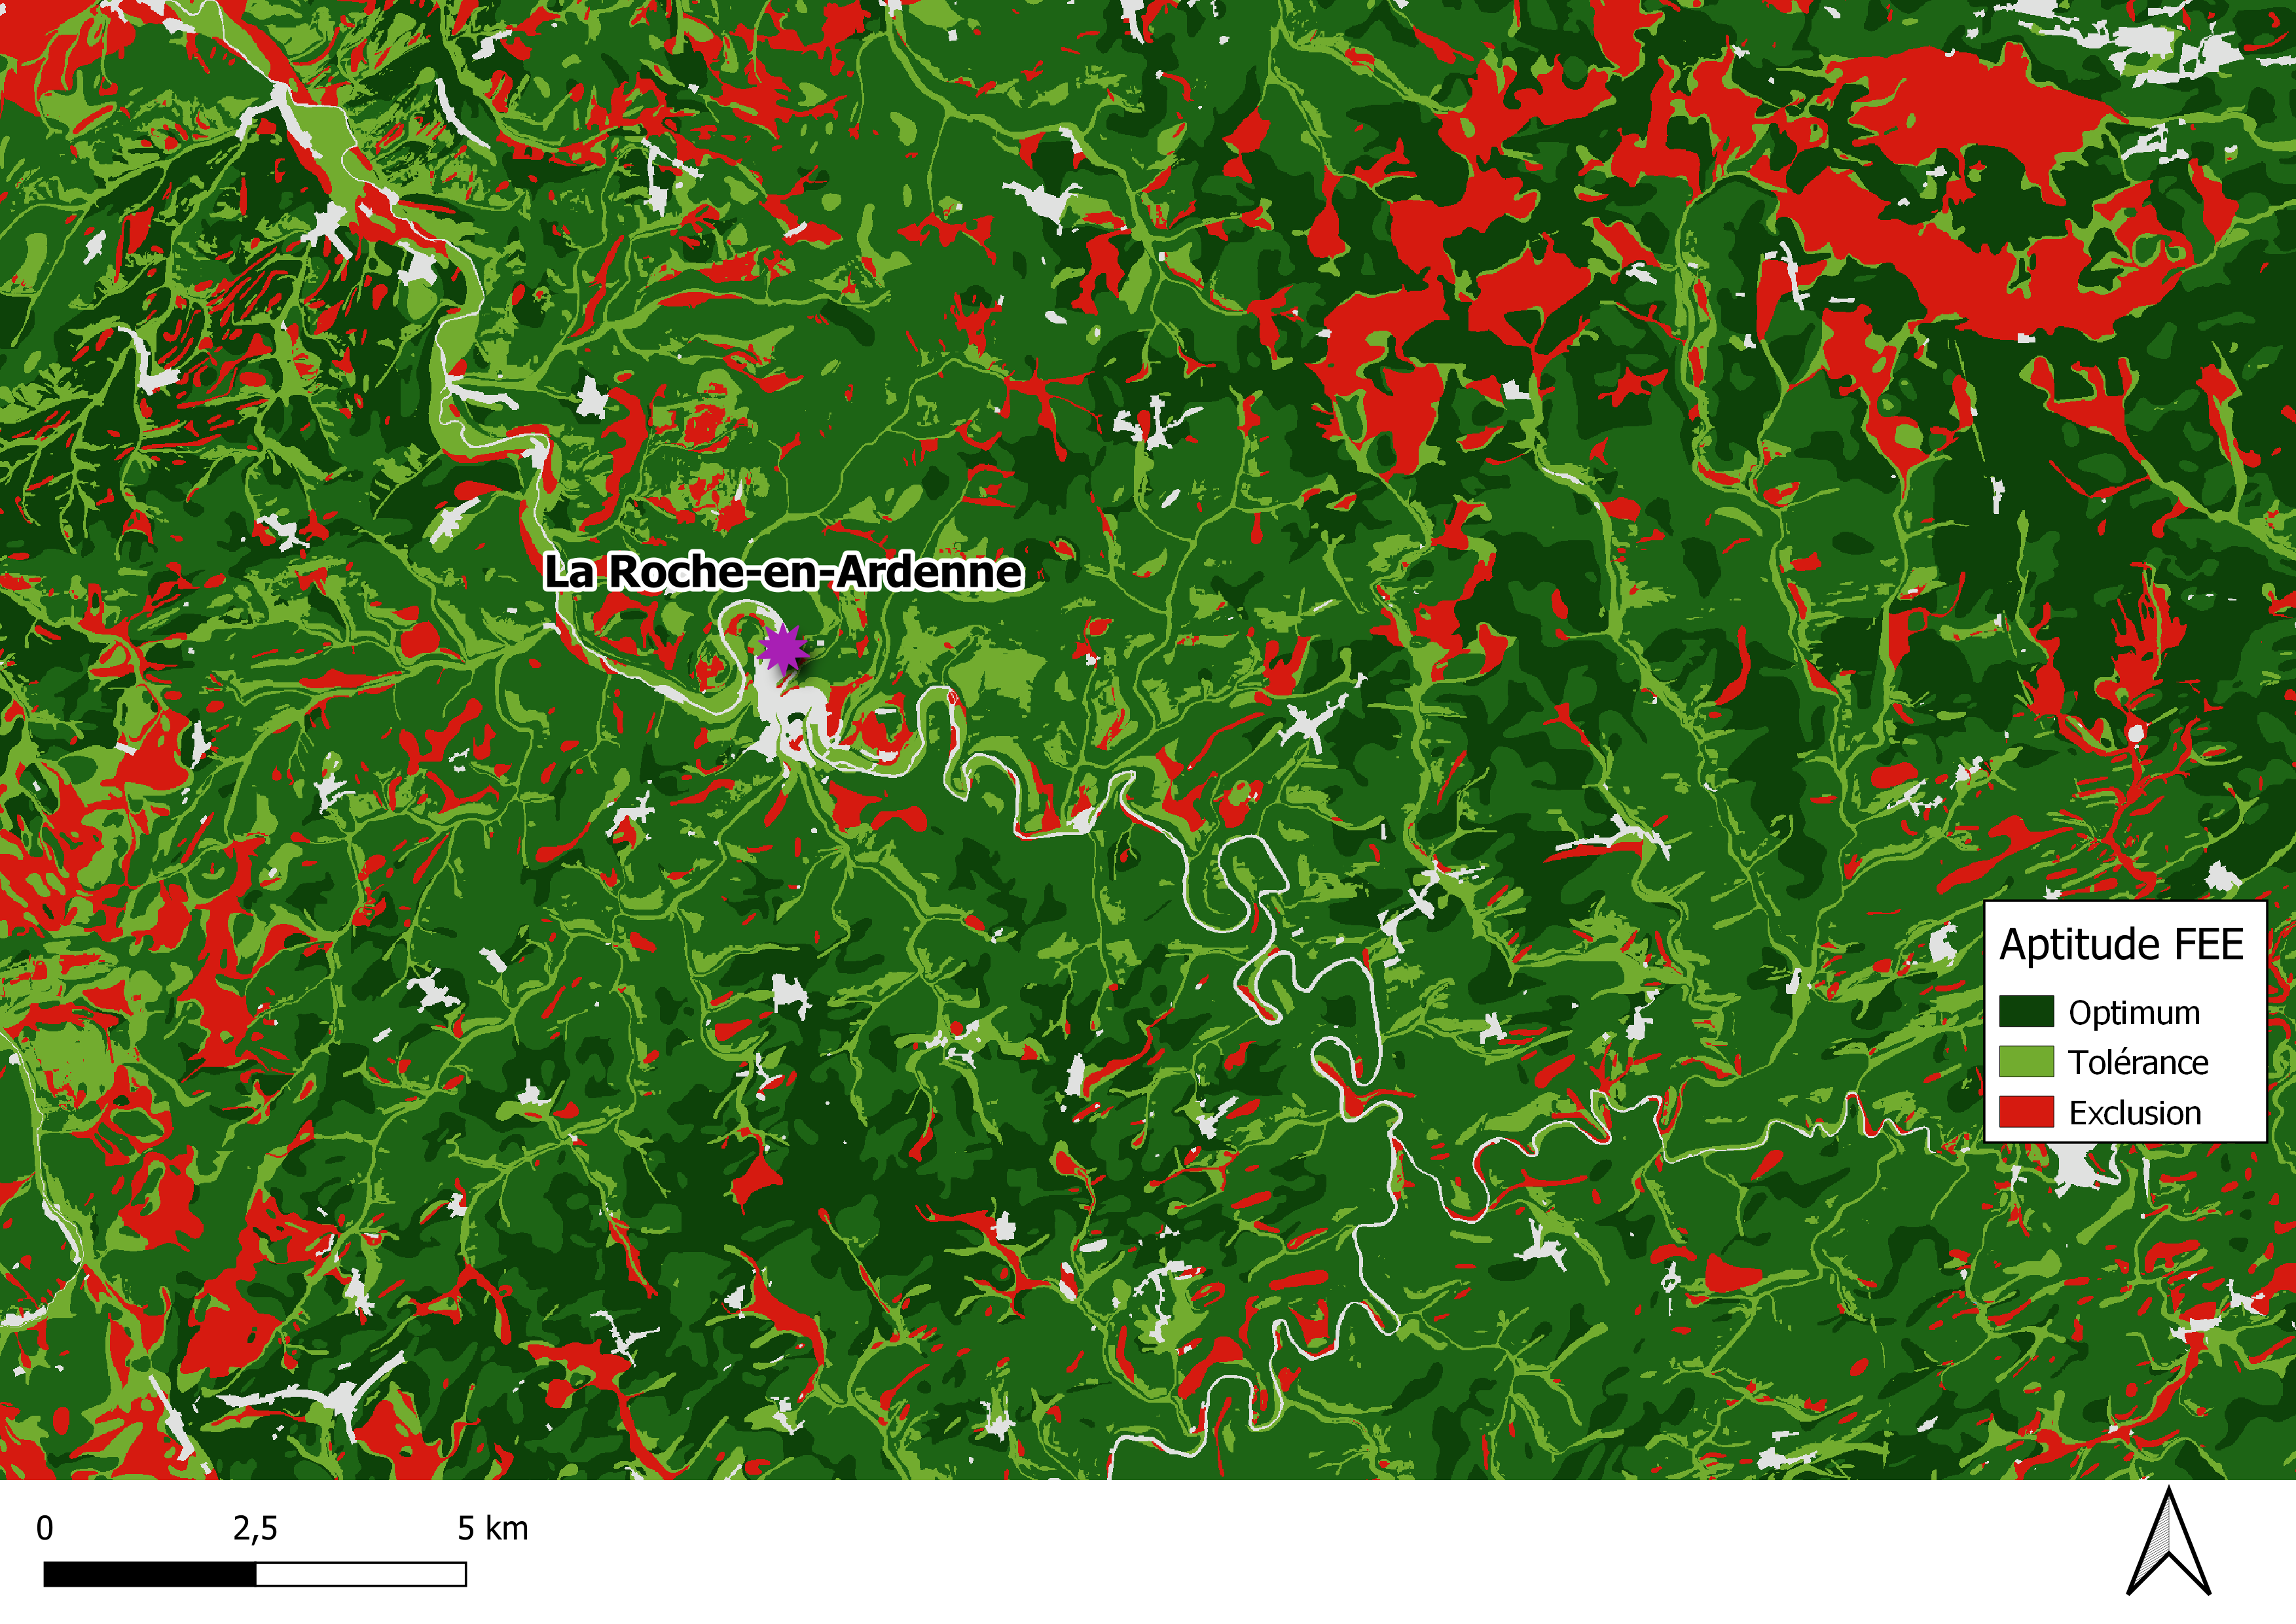
\includegraphics[width=1\textwidth]{exemple_laroche.png}
		\caption{Carte d'aptitude du Fichier Écologique des Essences sur la commune de la Roche-en-Ardenne. La teinte verte intermédiaire est une indétermination de l'aptitude (entre tolérance et optimum) qui ne peut être levée que par une analyse chimique du sol. }
		\label{fig: la_roche_1}
		
	\end{minipage}\hfill
	\vspace{1cm}
	\begin{minipage}[b]{1 \linewidth}
		\centering
		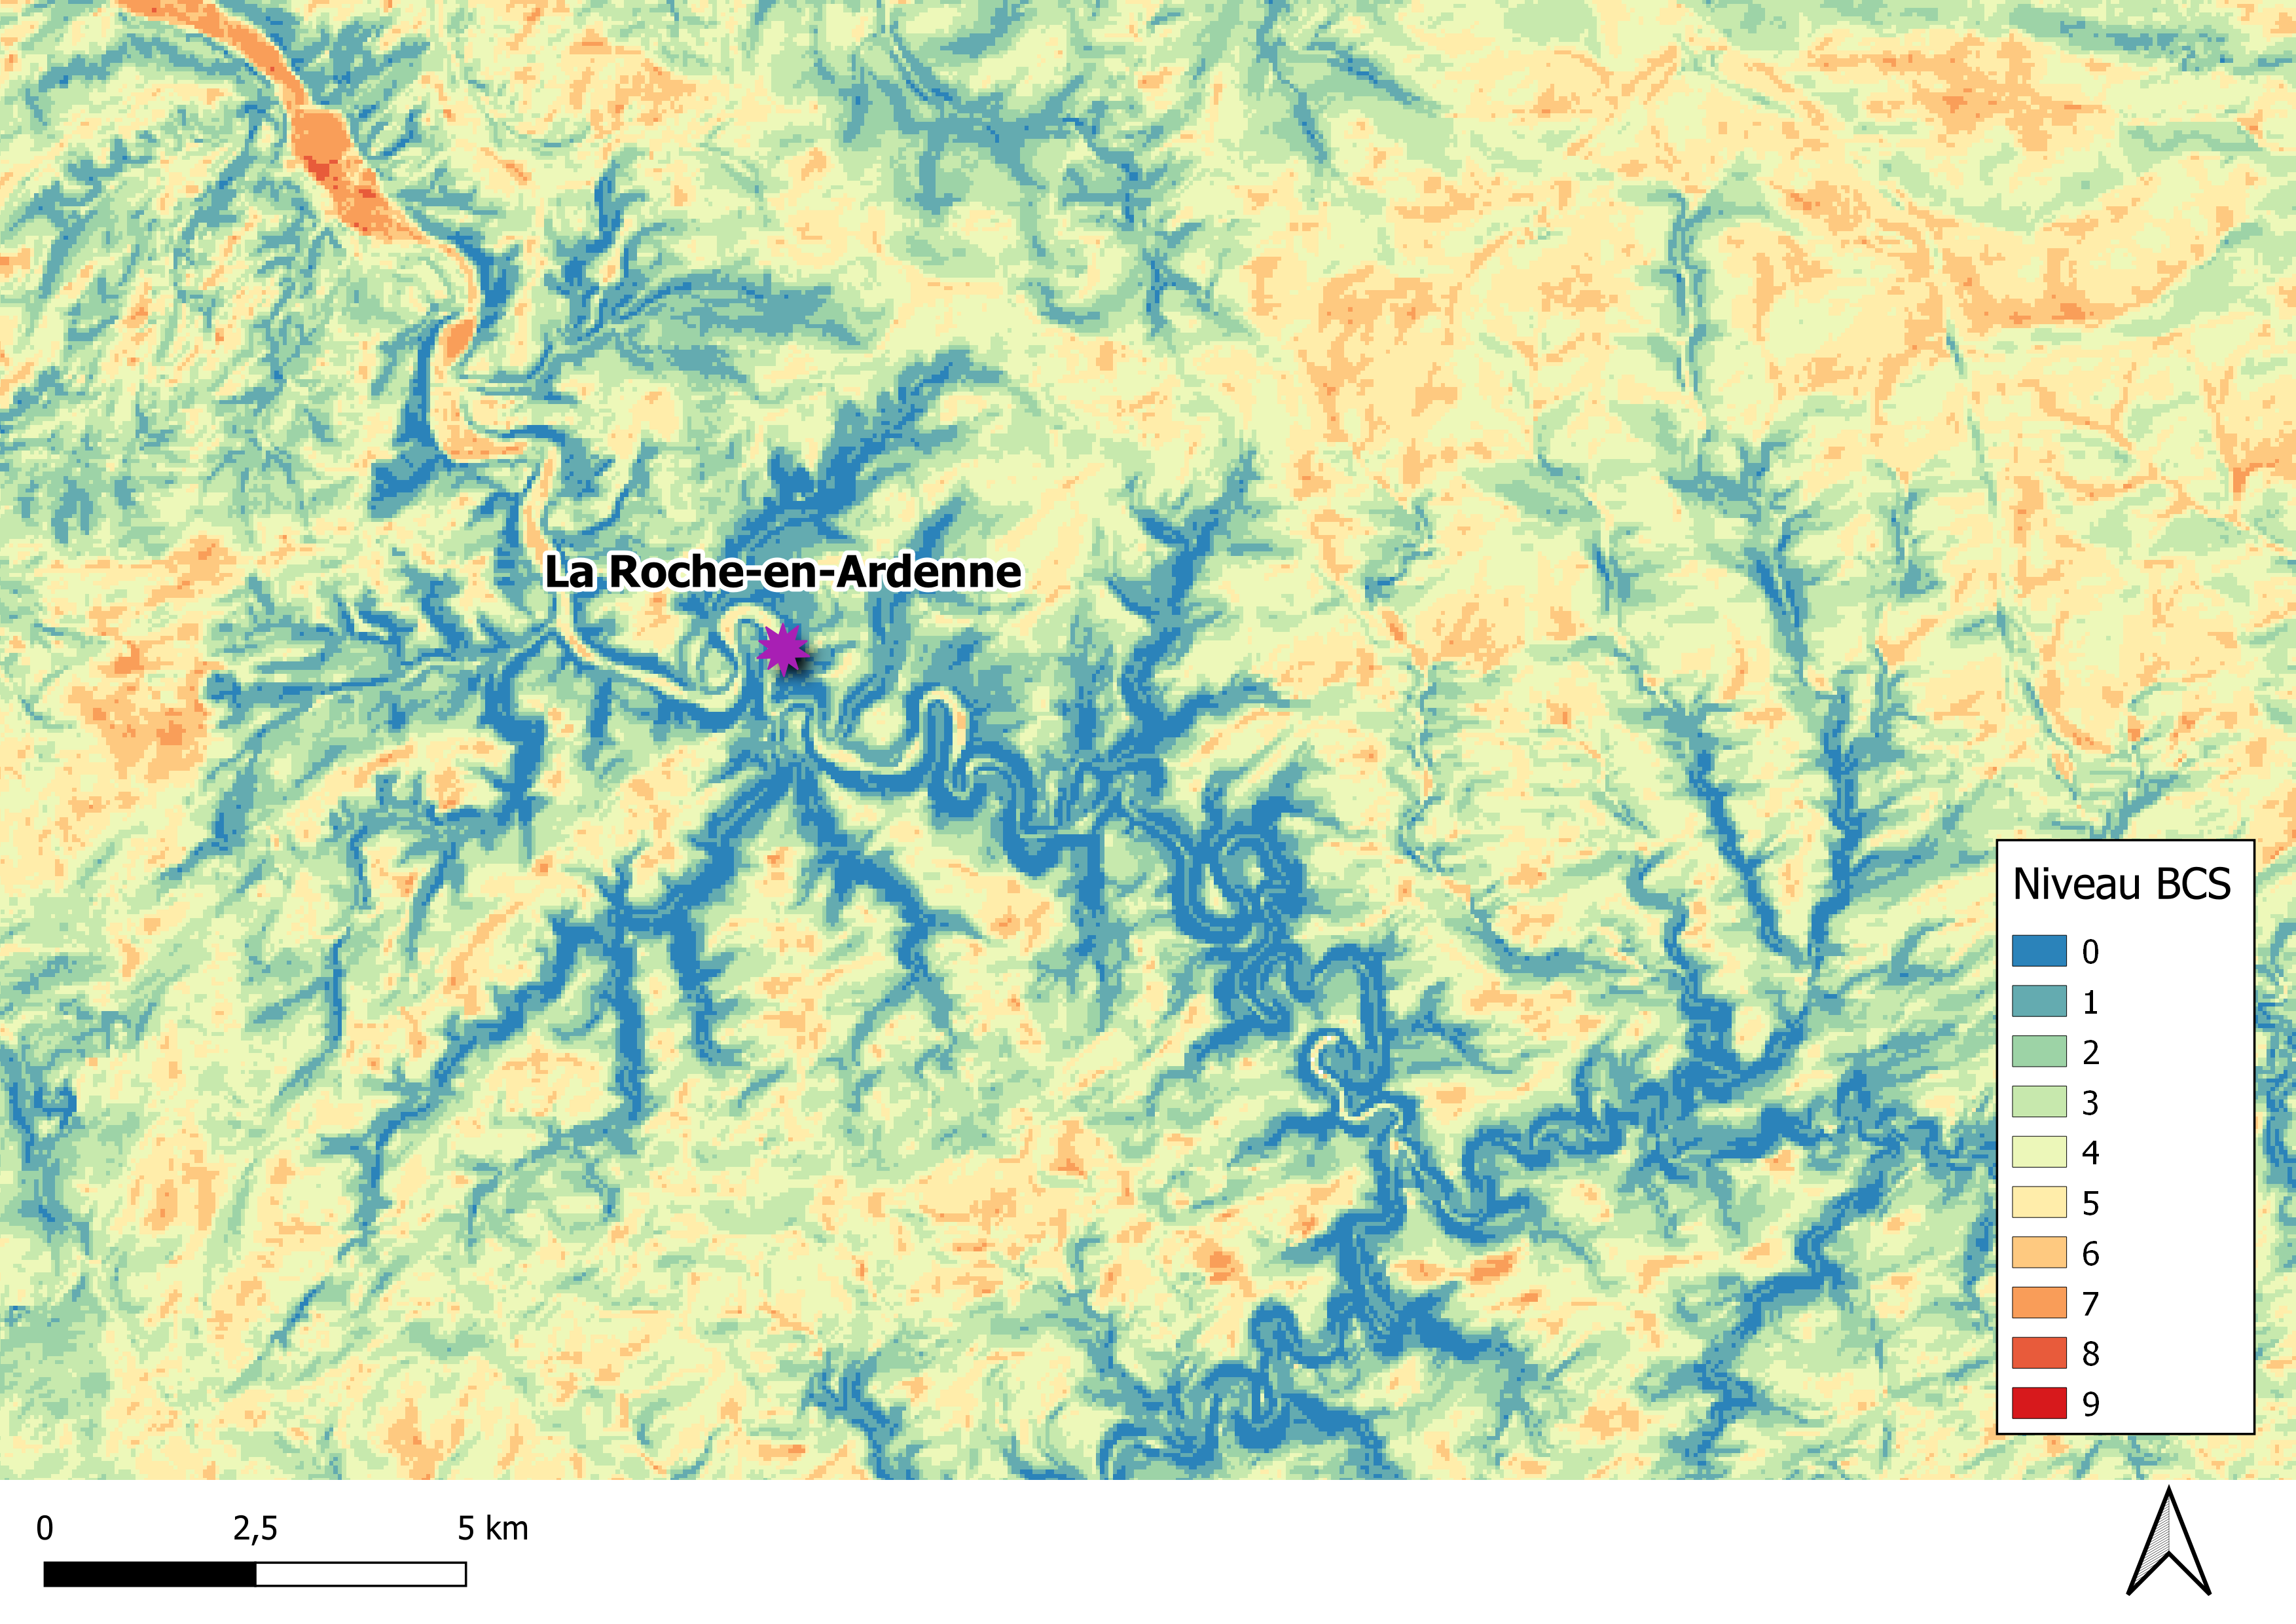
\includegraphics[width=1\textwidth]{exemple_laroche_BCS.png}
		\caption{Carte de risque d'attaque de scolytes issue du modèle BioClimSol sur la commune de la Roche-en-Ardenne.}
		\label{fig: la_roche_2}
	\end{minipage}
\end{figure}

\newpage
\subsection{Comparaison des méthodes.}

\subsubsection{Comparaison des cartes}
A l'échelle de la Wallonie les deux méthodes ont une certaine cohérence. Les deux cartes identifient nettement l'Ardenne comme une zone favorable à l'épicéa (optimale ou à faible risque) et le nord du sillon Sambre et Meuse comme une zone à haut risque ou d'exclusion.\\

Cependant, à une échelle plus fine , la carte de risque de BioClimSol et la carte d'aptitude du Fichier Écologique des Essences divergent fortement:


\begin{itemize}
	\item  le Fichier Écologique des Essences indique l'épicéa en optimum sur les plateaux de l'Ardenne, à l'exception des zones humides (tourbières et sols très hydromorphes), alors que BioClimSol y indique un risque élevé (5 à 7) partout.
	\item BioClimSol considère le risque quasi nul (0 ou 1) dans les grands versants, quelque soit leur exposition ou rayonnement, là ou le Fichier Écologique des Essences est plus mitigé en identifiant les versants chauds comme des situations de tolérance.
\end{itemize}

\subsubsection{Confrontation des cartes de risque et d'aptitude à la probabilité de présence d'arbres scolytés}

Les niveaux de risque et d'aptitude ont été ensuite confrontés à la probabilité de présence d'épicéas scolytés estimée à l'aide de l'imagerie satellitaire. \\

Pour comparer les deux méthodes, les niveaux de risque de BioClimSol ont été traduits en trois niveaux d'aptitude pour l'épicéa (Tableau \ref{tab: level}).

\begin{table}[htbp]
	\caption{Conversion des différents niveaux BioClimSol en niveau d'aptitude}
	\label{tab: level}
	\begin{tabular}{|l|l|}
		\hline
		Niveau d'aptitude & Niveau BioClimSol \\ \hline
		Optimum           & $<2$            \\ \hline
		Tolérance         & 2 à 4          \\ \hline
		
		Exclusion         &  $>4$   \\ \hline
	\end{tabular}
	
\end{table}
\begin{figure}[htbp]
	\begin{minipage}[b]{1 \linewidth}
		\centering
		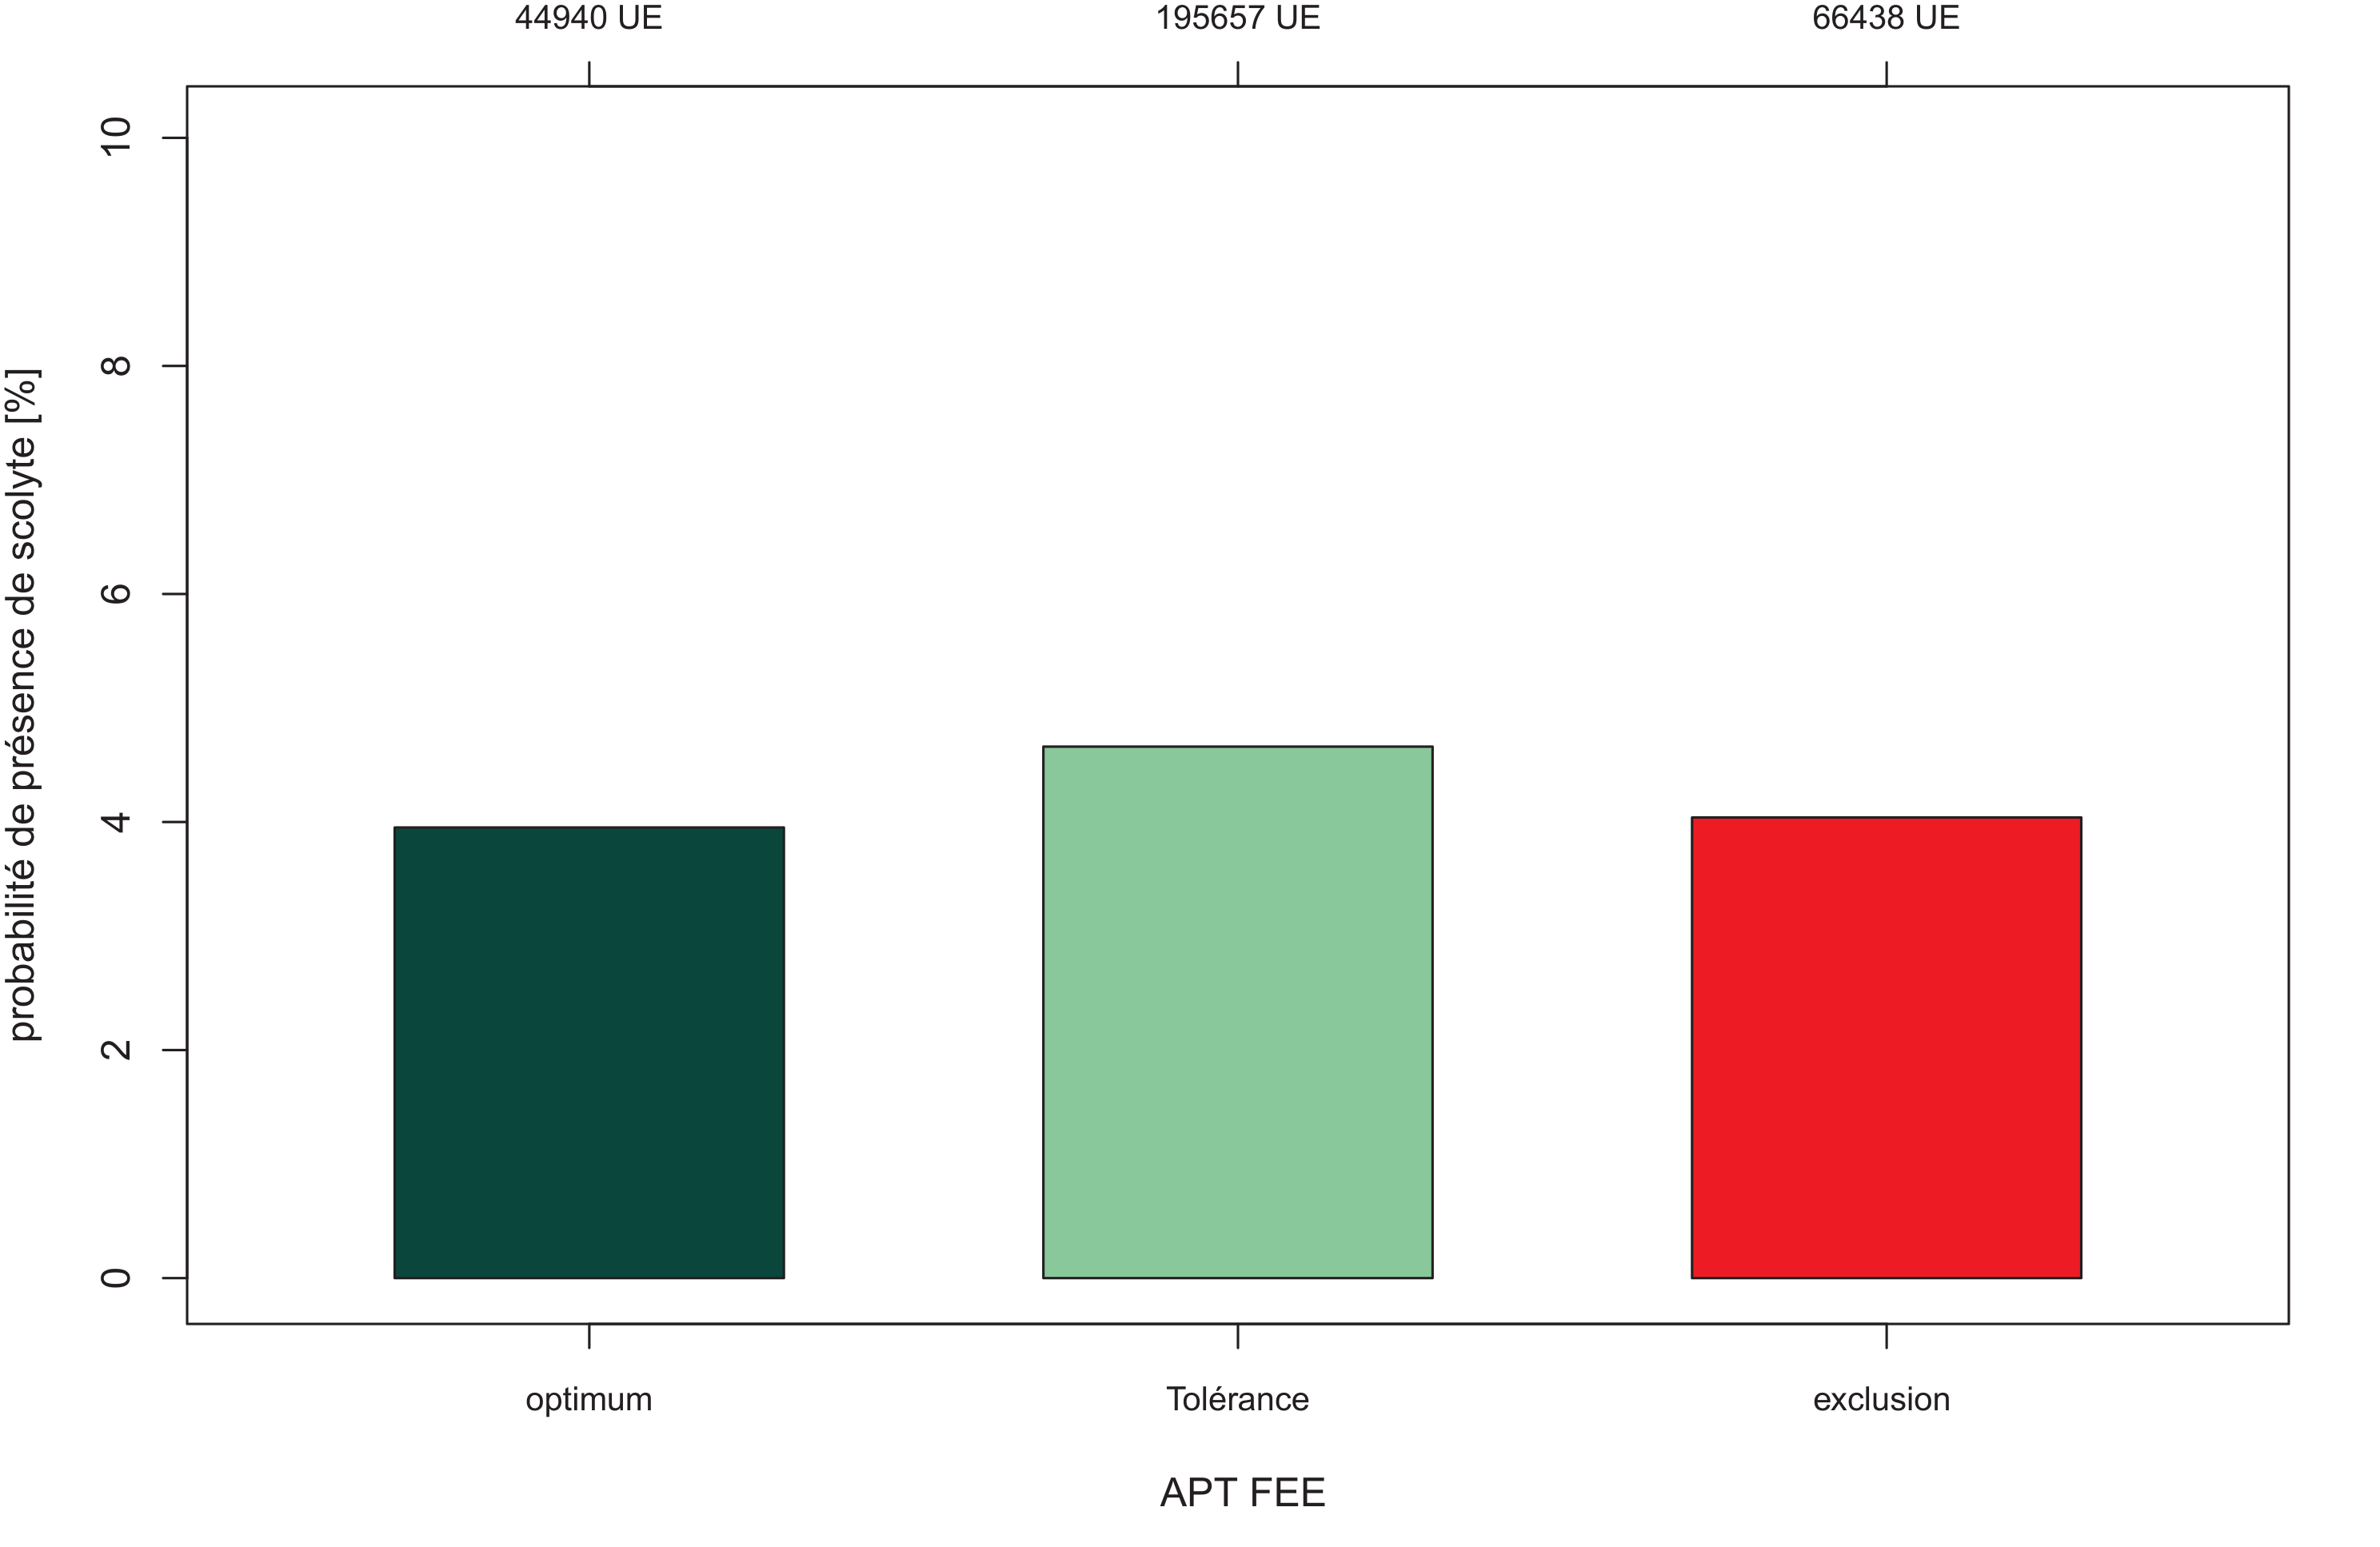
\includegraphics[width=1\textwidth]{presenceScolyte_par_niveau_FEEv2.png}
		\caption{Probabilité de présence de scolytes en fonction des aptitudes du Fichier Écologiques des Essences }
		\label{fig: FEE}
		
	\end{minipage}\hfill
	\vspace{2cm}
	\begin{minipage}[b]{1 \linewidth}
		\centering
		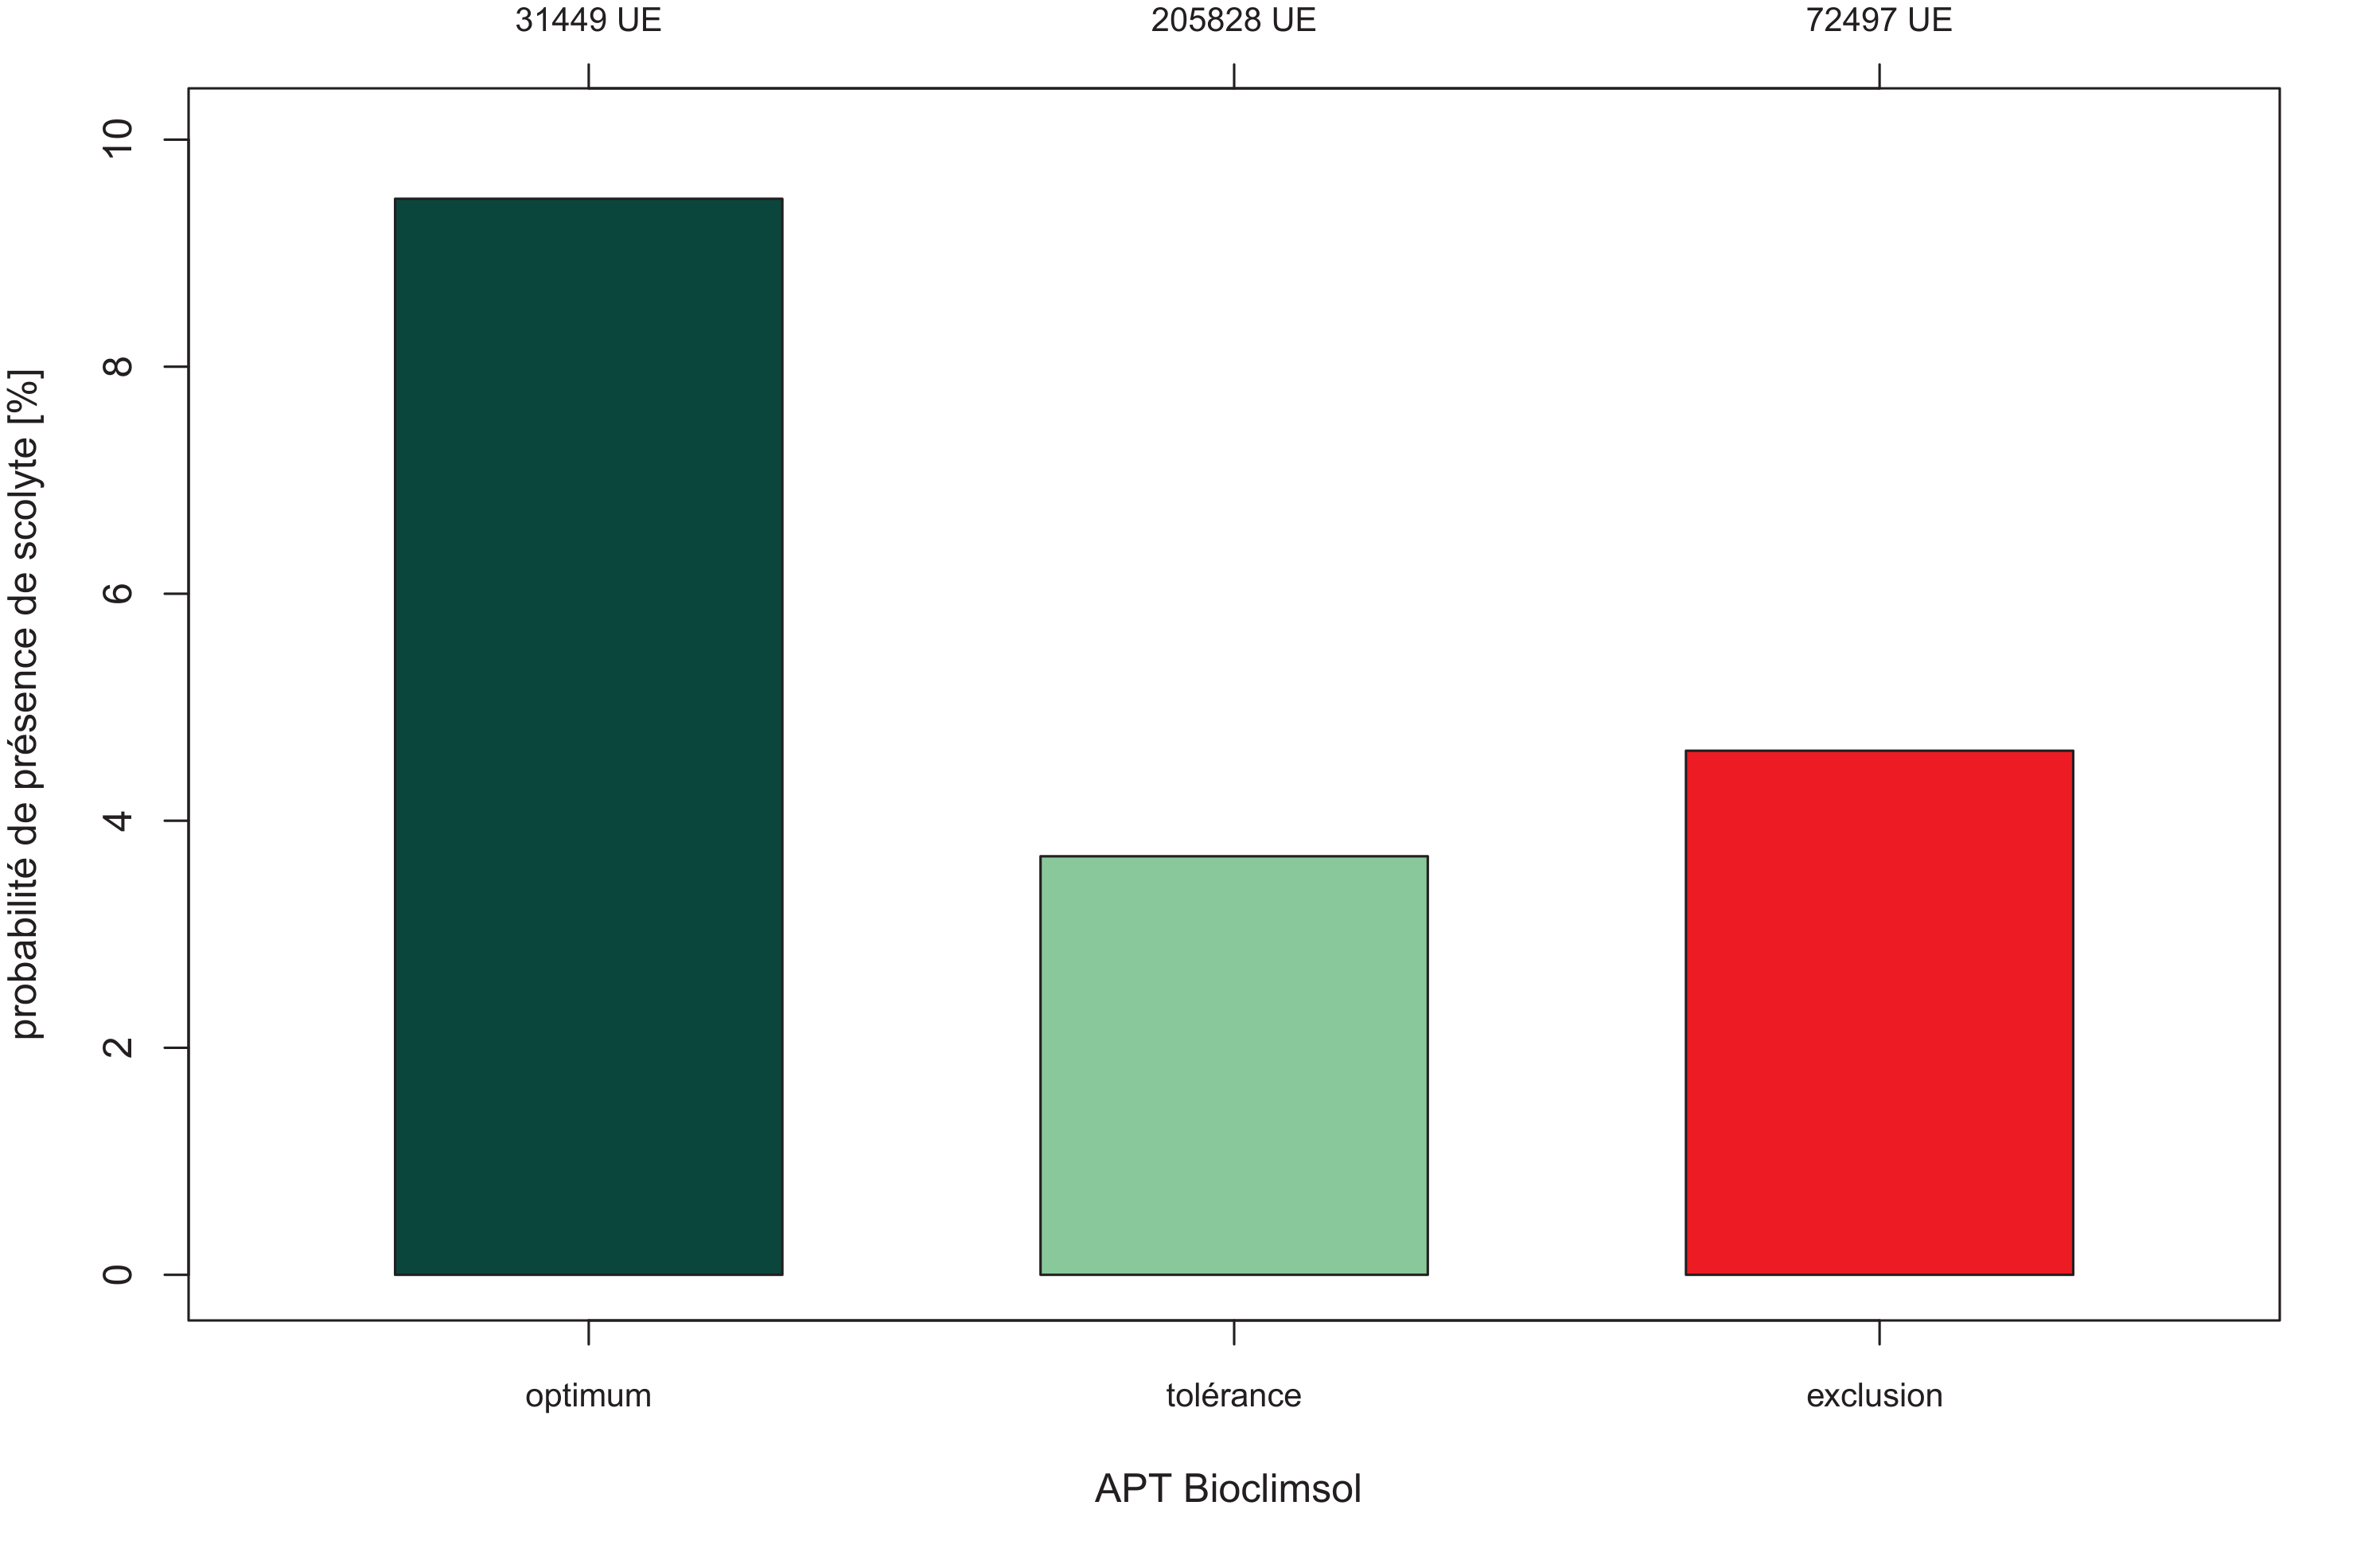
\includegraphics[width=1\textwidth]{presenceScolyte_par_niveau_Bioclimsol.png}
		\caption{Probabilité de présence de scolytes en fonction des aptitudes de BioClimSol}
		\label{fig: apt_2}
	\end{minipage}
\end{figure}

La comparaison de la probabilité de présence de scolyte en fonction des classe d’aptitude du Fichier Écologique des essences (Figure \ref{fig: FEE}) et du modèle de risque pour l'épicéa de BioClimSol (Figure \ref{fig: apt_2}) montre que pour le modèle BioClimSol, la probabilité de présence de scolytes est deux fois plus élevée en optimum que dans les autres classes d’aptitude tandis que cette probabilité est relativement similaire (aux alentours de 4\%) pour les trois classes de la carte d'aptitude du Fichier Écologique des Essences pour l'épicéa.

\subsubsection{Analyses complémentaires}
Les différences de comportement des modèles en fonction de la position topographique nous ont menés à analyser plus en détail les attaques de scolytes selon l'altitude et l'orientation des versants, et à élargir l'analyse aux Vosges. L'estimation de la probabilité d'attaques de scolytes a été menée selon la même méthodologie dans les Vosges, puis mise en relation avec l'altitude et la position topographique.\\

Pour l'année 2020, l'augmentation de la probabilité de présence de scolyte continue encore dans les pessières présentes en dessous de 400 m d'altitude alors qu'elle reste en dessous de cinq pourcent au dessus de 400m d'altitude.\\

En Wallonie, l'altitude influence donc fortement les attaques de scolytes. Plus l'altitude augmente, plus la probabilité de présence de scolyte diminue. \\

\begin{figure}[htbp]
	\begin{minipage}[b]{1 \linewidth}
		\centering
		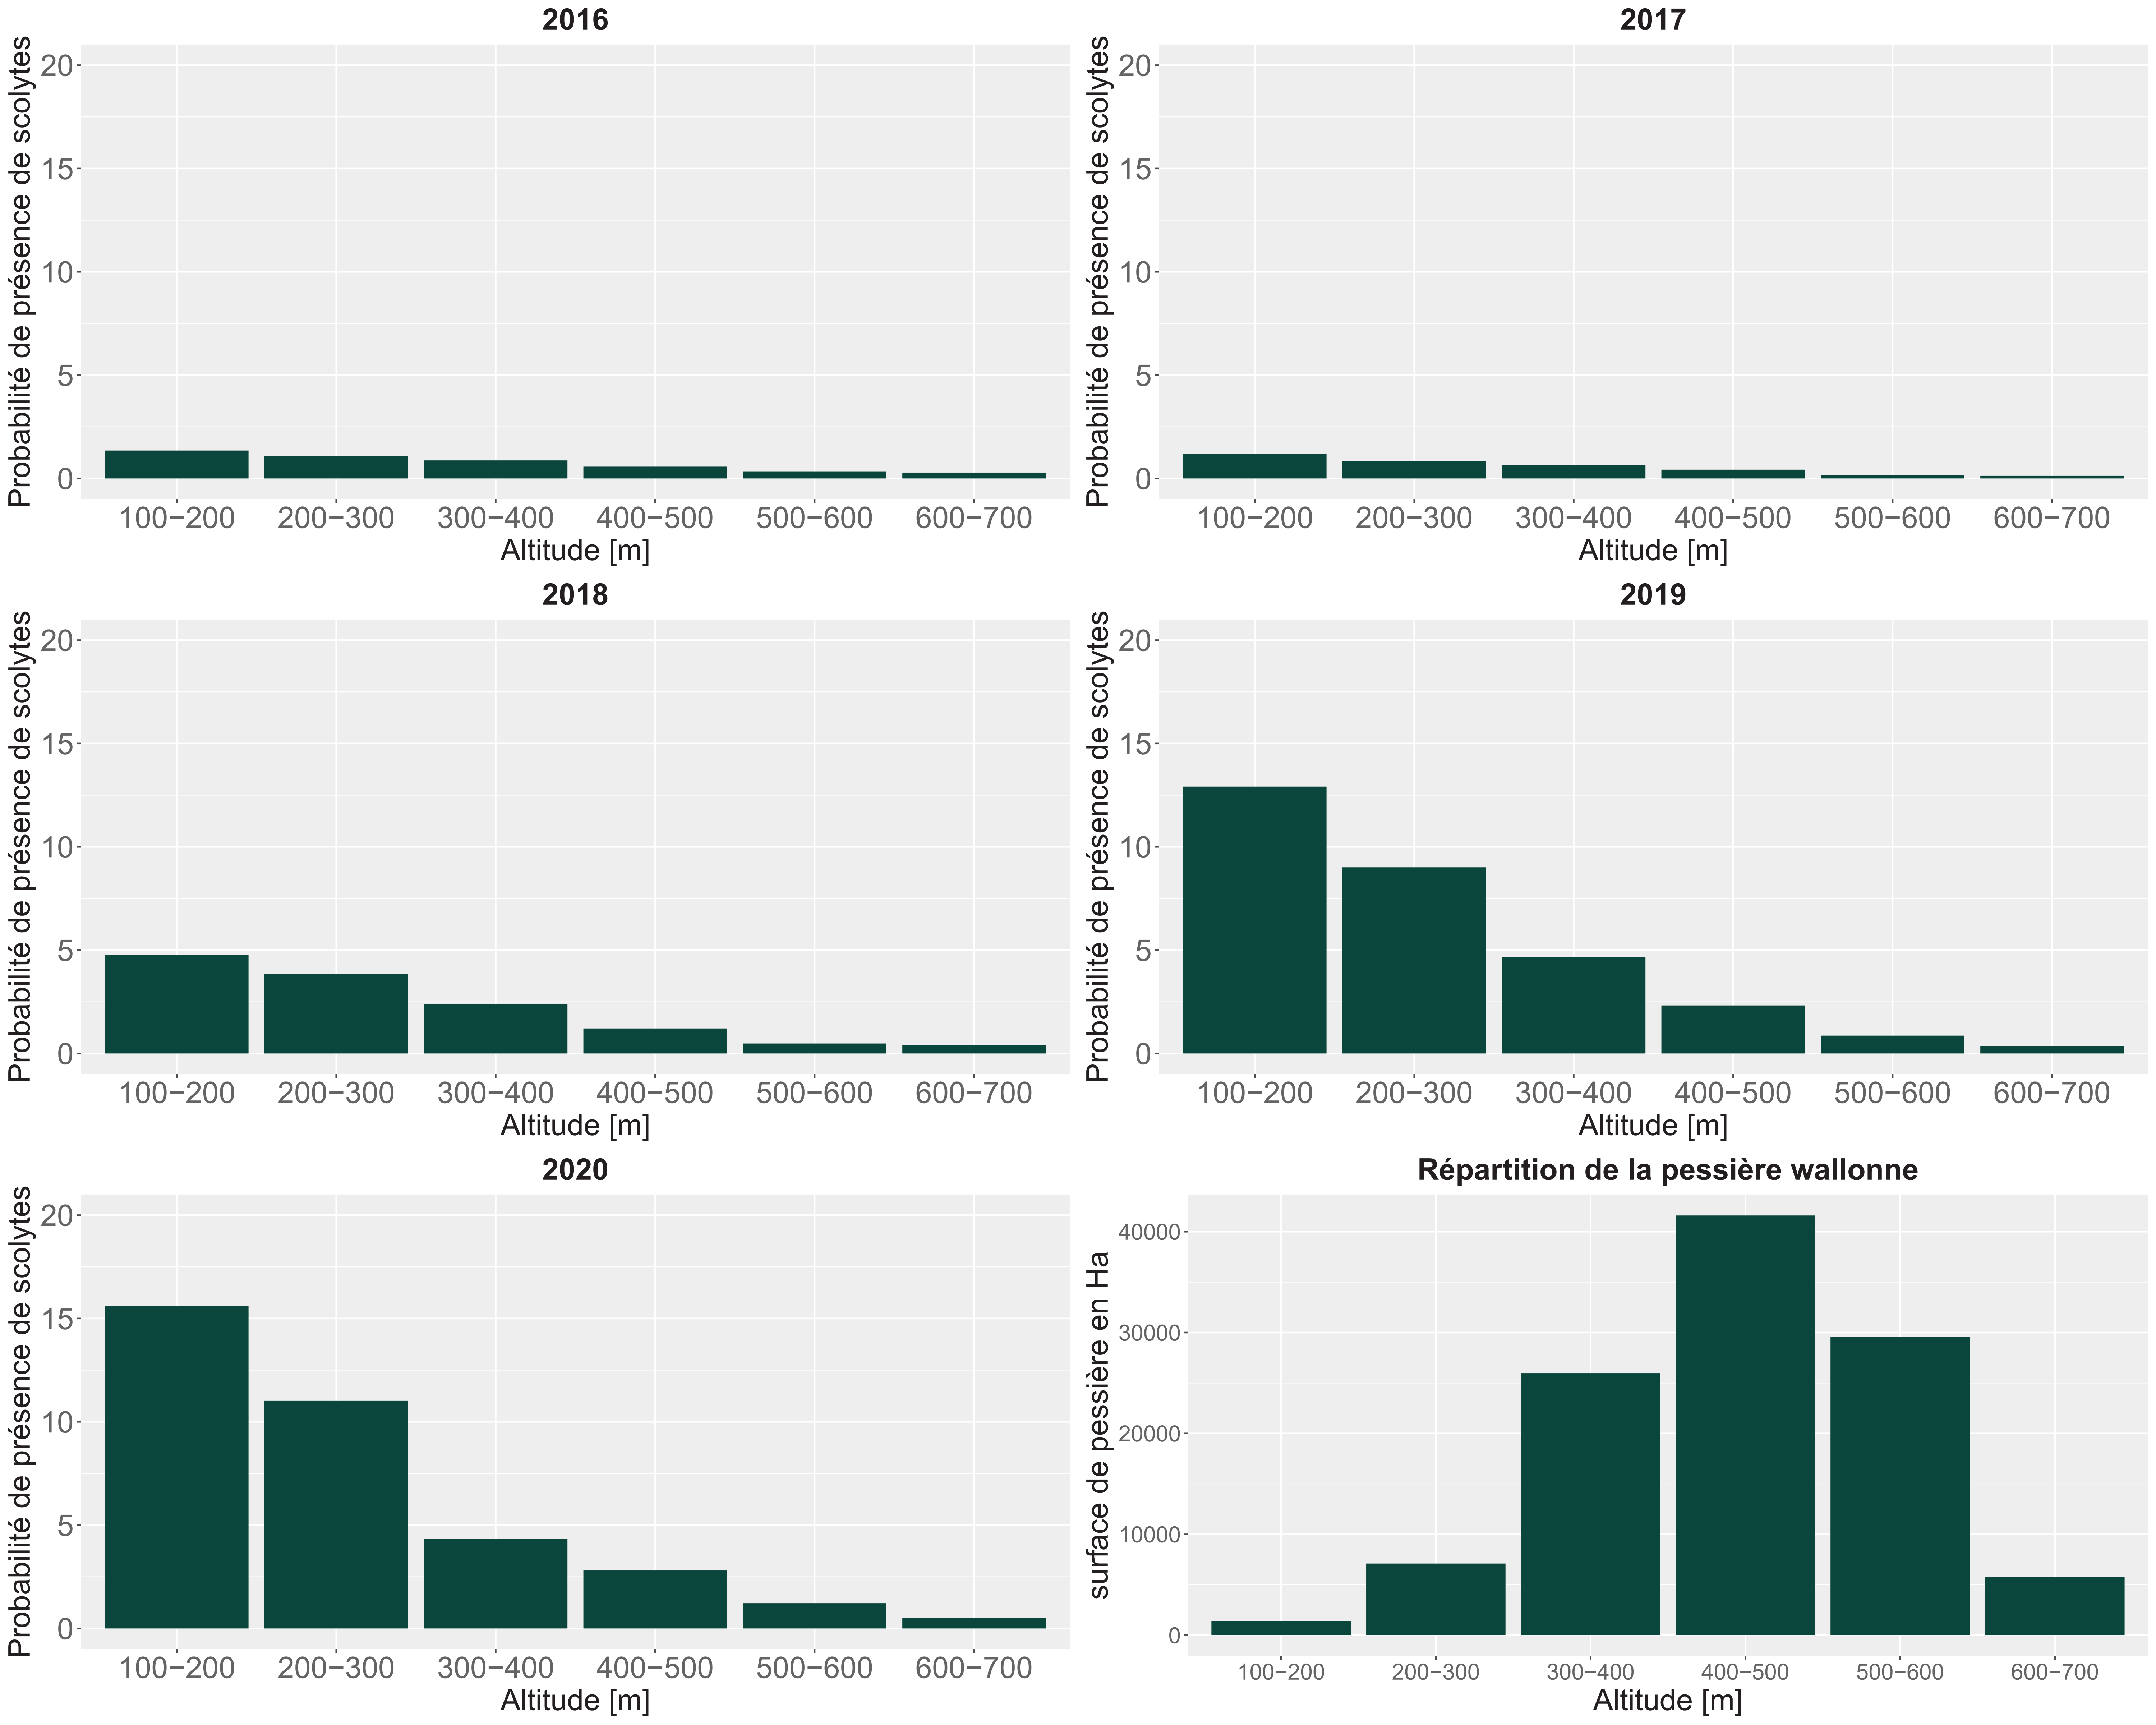
\includegraphics[width=0.9\textwidth]{alti_wal.png}
		\caption{Évolution temporelle de la crise du typographe en fonction de l'altitude des pessières en Wallonie }
		\label{fig: alti_rw}
		
	\end{minipage}\hfill
	\vspace{0.75cm}
	\begin{minipage}[b]{1 \linewidth}
		\centering
		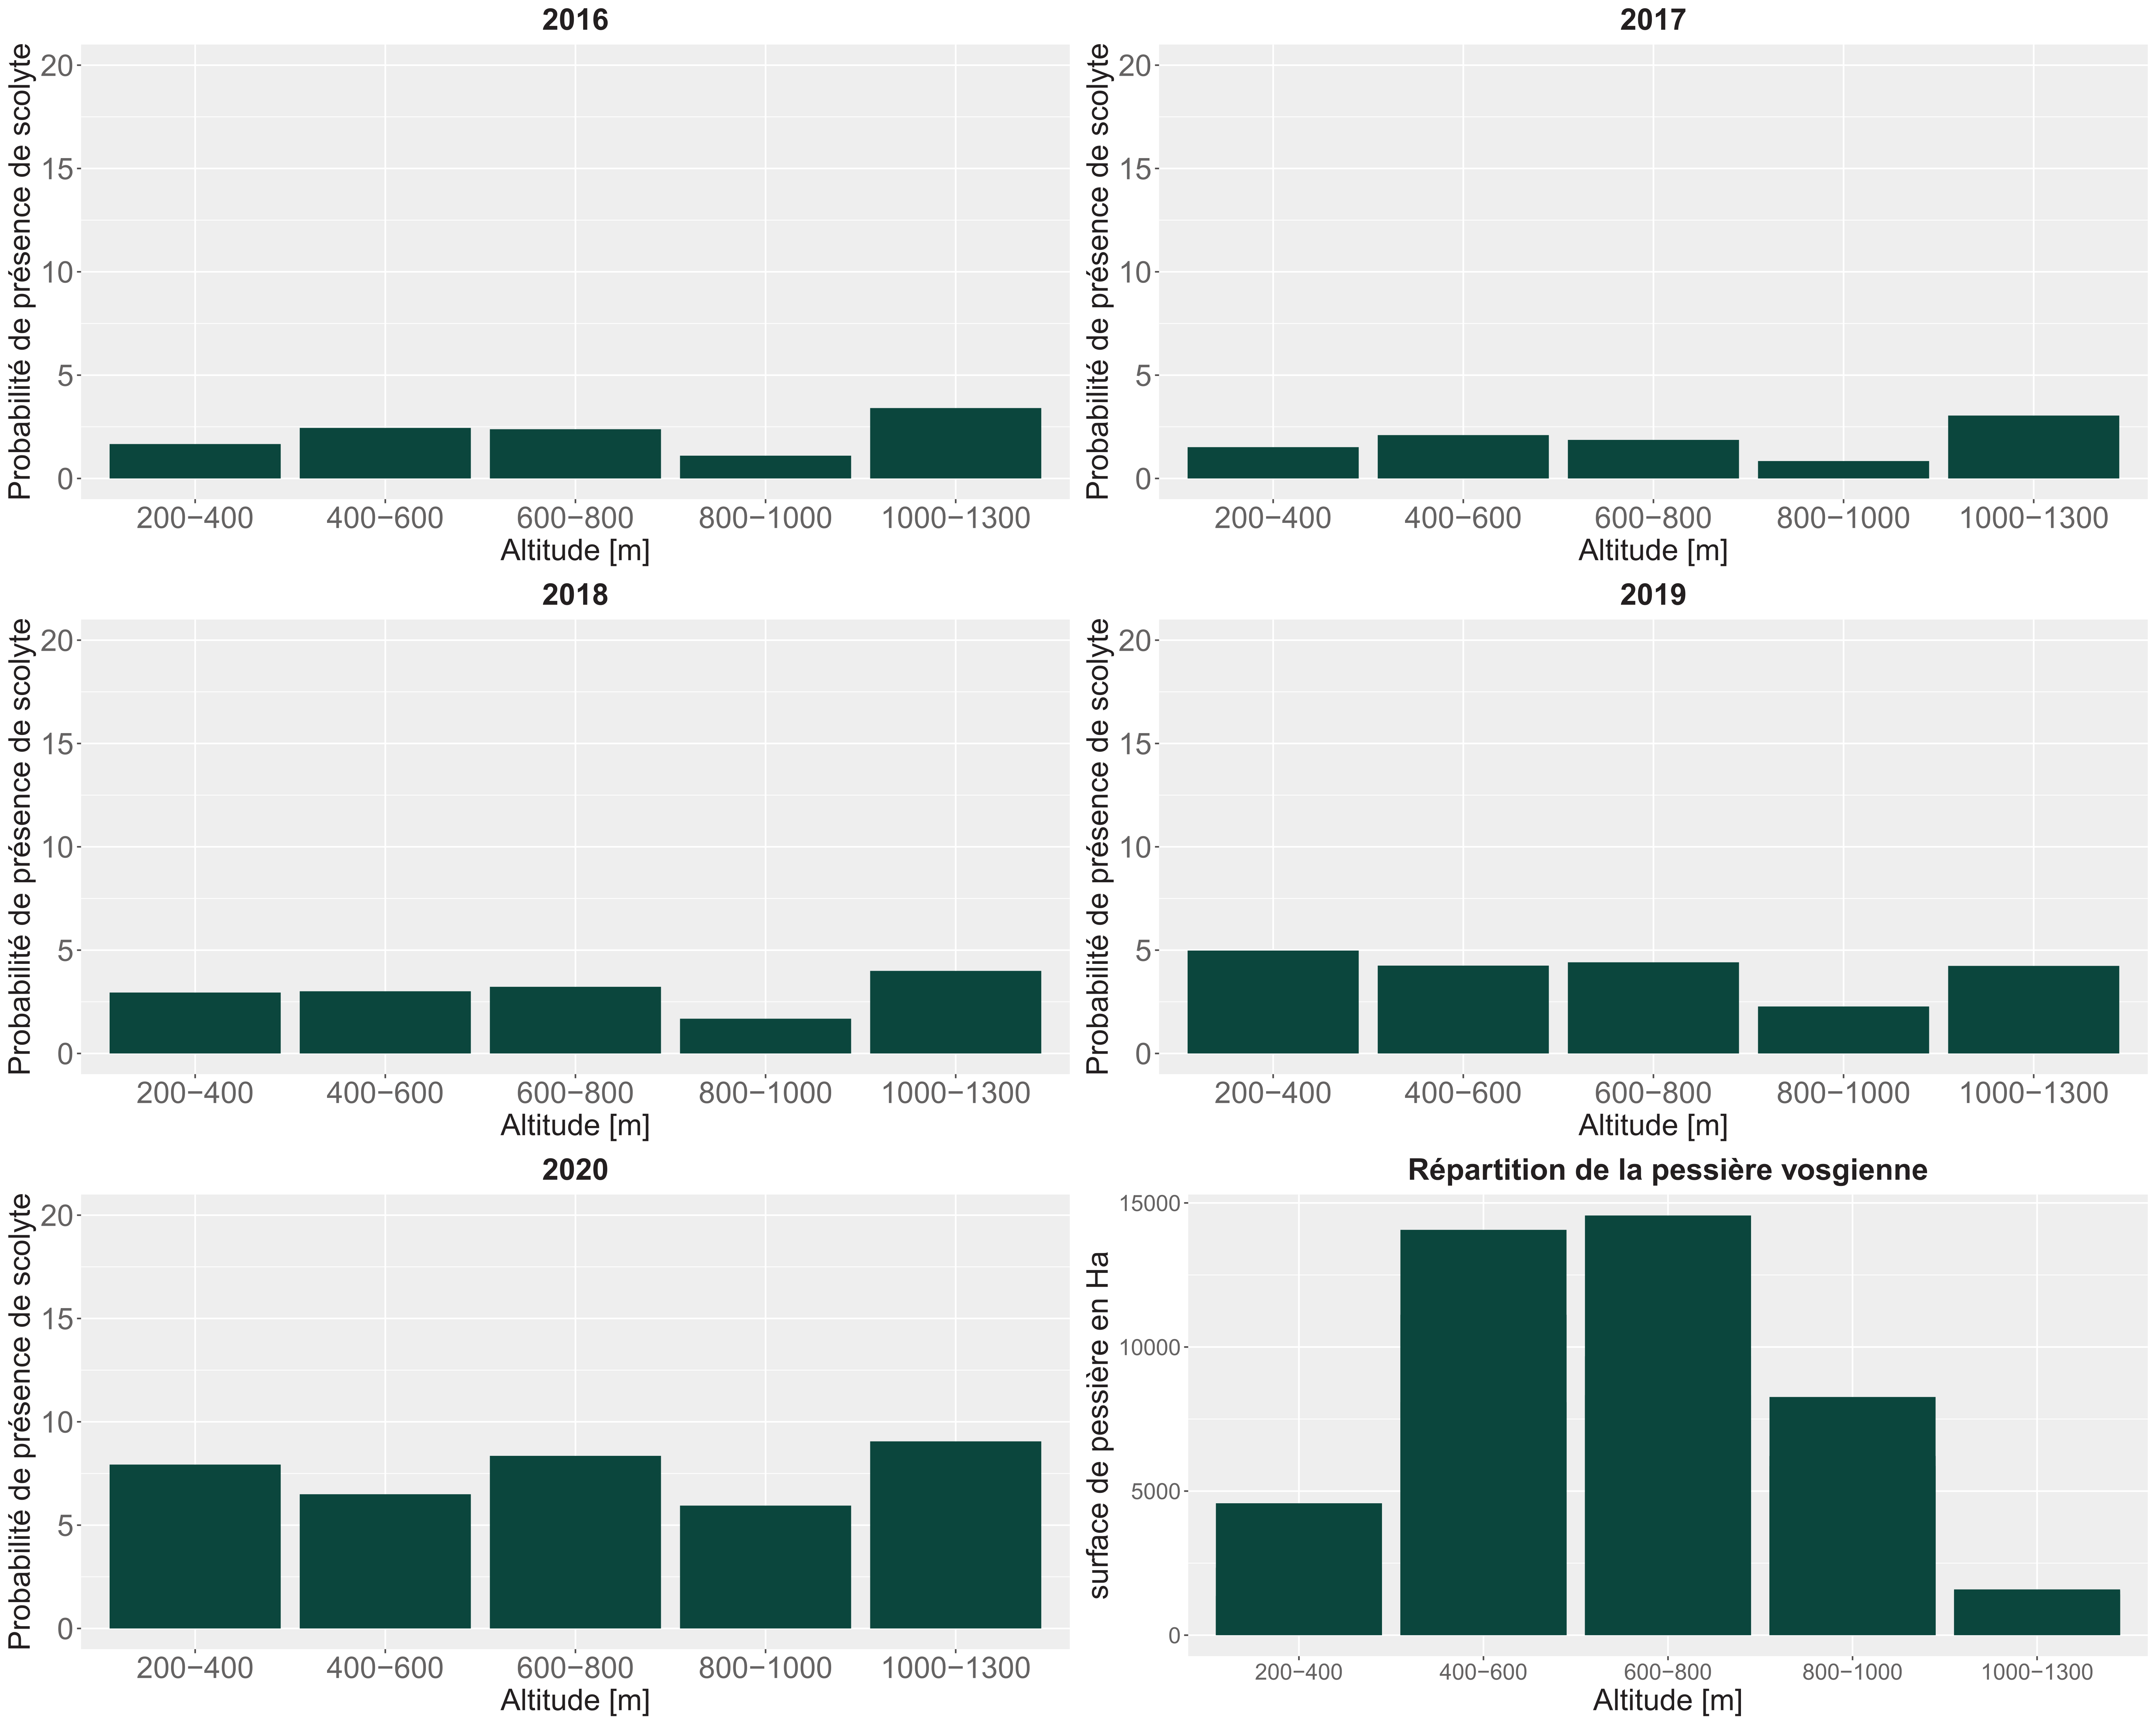
\includegraphics[width=0.9\textwidth]{alti_vosge.png}
		\caption{Évolution temporelle de la crise du typographe dans les Vosges en fonction de l'altitude.}
		\label{fig: alti_vosges}
	\end{minipage}
\end{figure}




La majorité de la pessière vosgienne se situe dans les classes d'altitudes situées entre 400 et 800m (figure \ref{fig: alti_vosges}).
La figure \ref{fig: alti_vosges} montre que la probabilité de présence de scolyte dans les Vosges ne semble pas influencée par l'altitude. Jusqu'en 2019, la probabilité de présence de scolyte reste relativement stable et inférieure à 5 pourcent. En 2020, une augmentation de la probabilité de présence se produit, la barre de 5 pourcent de probabilité est franchie. Cependant quelque soit la classe d'altitude, cette probabilité reste inférieure à 10 pourcent.


La probabilité de présence de scolytes ne semble donc pas liée au gradient altitudinal dans les Vosges.


\subsubsection{Topographie}
Afin de comparer la probabilité de présence de scolyte selon les pentes des Vosges et en Wallonie, un raster sous-secteur a été calculé pour la tuile Sentinel 2 T32ULU. La méthodologie utilisée pour déterminer les sous-secteurs sur la tuile Sentinel 2 T32ULU est identique à celle employée pour le Fichier Écologique des essences \citep{wampach_cartographie_2017}.

Concernant les pentes, le fichier écologique suggère une situation favorable pour l'épicéa dans les versant nord (sous-secteur froid) et un risque élevé dans les versants sud ( sous-secteur chaud). Les faibles pentes (< 20\%) et les plateaux sont considérés comme ayant un risque faible pour cette essence (figure \ref{fig:ficheco}).

D'après le Fichier Ecologique des Essences, l'épicéa court un risque élevé en dessous de 200 m d'altitude, un risque faible entre 200 et 350m et un risque absent au dessus de 350 m d'altitude (Figure \ref{fig:fichalti}).  

\begin{figure} [htbp] 
	\centering
	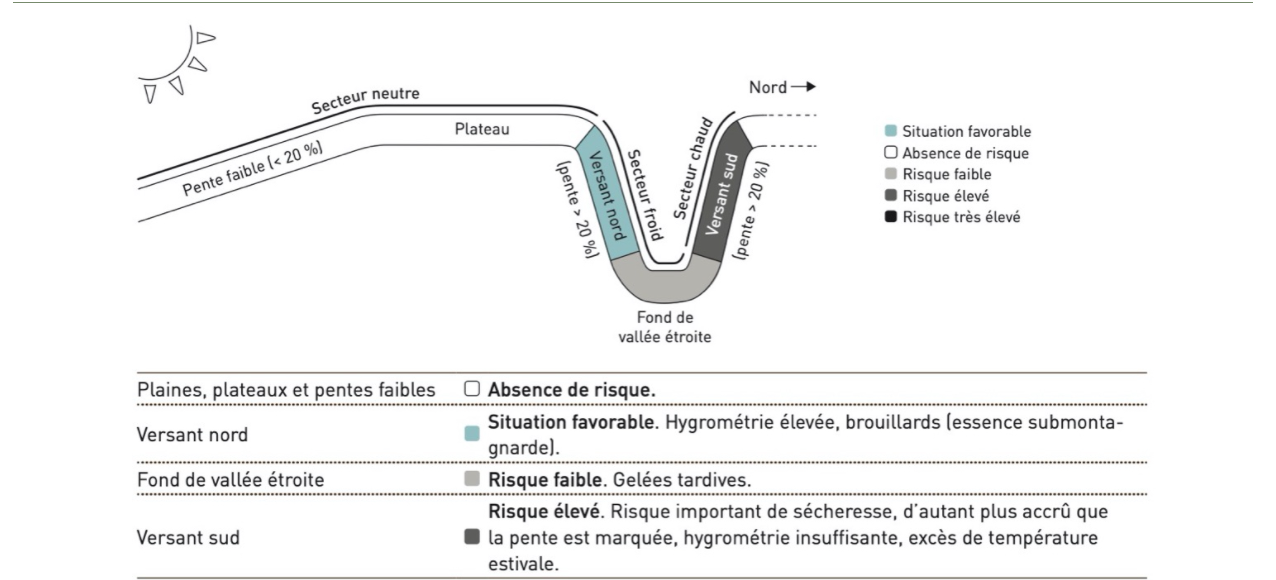
\includegraphics[width=1\textwidth]{illu_rapp.PNG}
	\caption{Risque pour l'épicéa en fonction de la topographie (fichierecologique.be)}
	\label{fig:ficheco}
\end{figure}

\begin{figure} [htbp] 
	\centering
	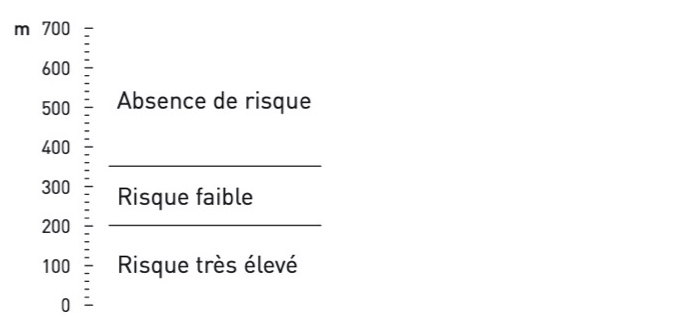
\includegraphics[width=0.8\textwidth]{EP320.png}
	\caption{Aptitude altitudinale de l'épicéa en Wallonie (fichierecologique.be)}
	\label{fig:fichalti}
\end{figure}

Le modèle de risque BioClimSol indique que l'épicéa risque moins de se faire attaquer par le typographe  dans les pentes.
Cependant, les premiers résultats des cartes de scolytes de 2016 à 2020 (Figure \ref{fig:topo}) montrent que pour la Wallonie, les épicéas sont significativement plus atteints (d'après un test de Student) dans les pentes (que ce soit les pentes nord ou les pentes sud ce qui diverge du Fichier Écologique) que sur les plateaux, ce qui ne se confirme pas significativement dans les Vosges.
Les versants nord de Wallonie sont significativement plus touchés que les versants sud de cette région. 

\begin{figure}[htbp]
	\begin{minipage}[b]{1 \linewidth}
		\centering
		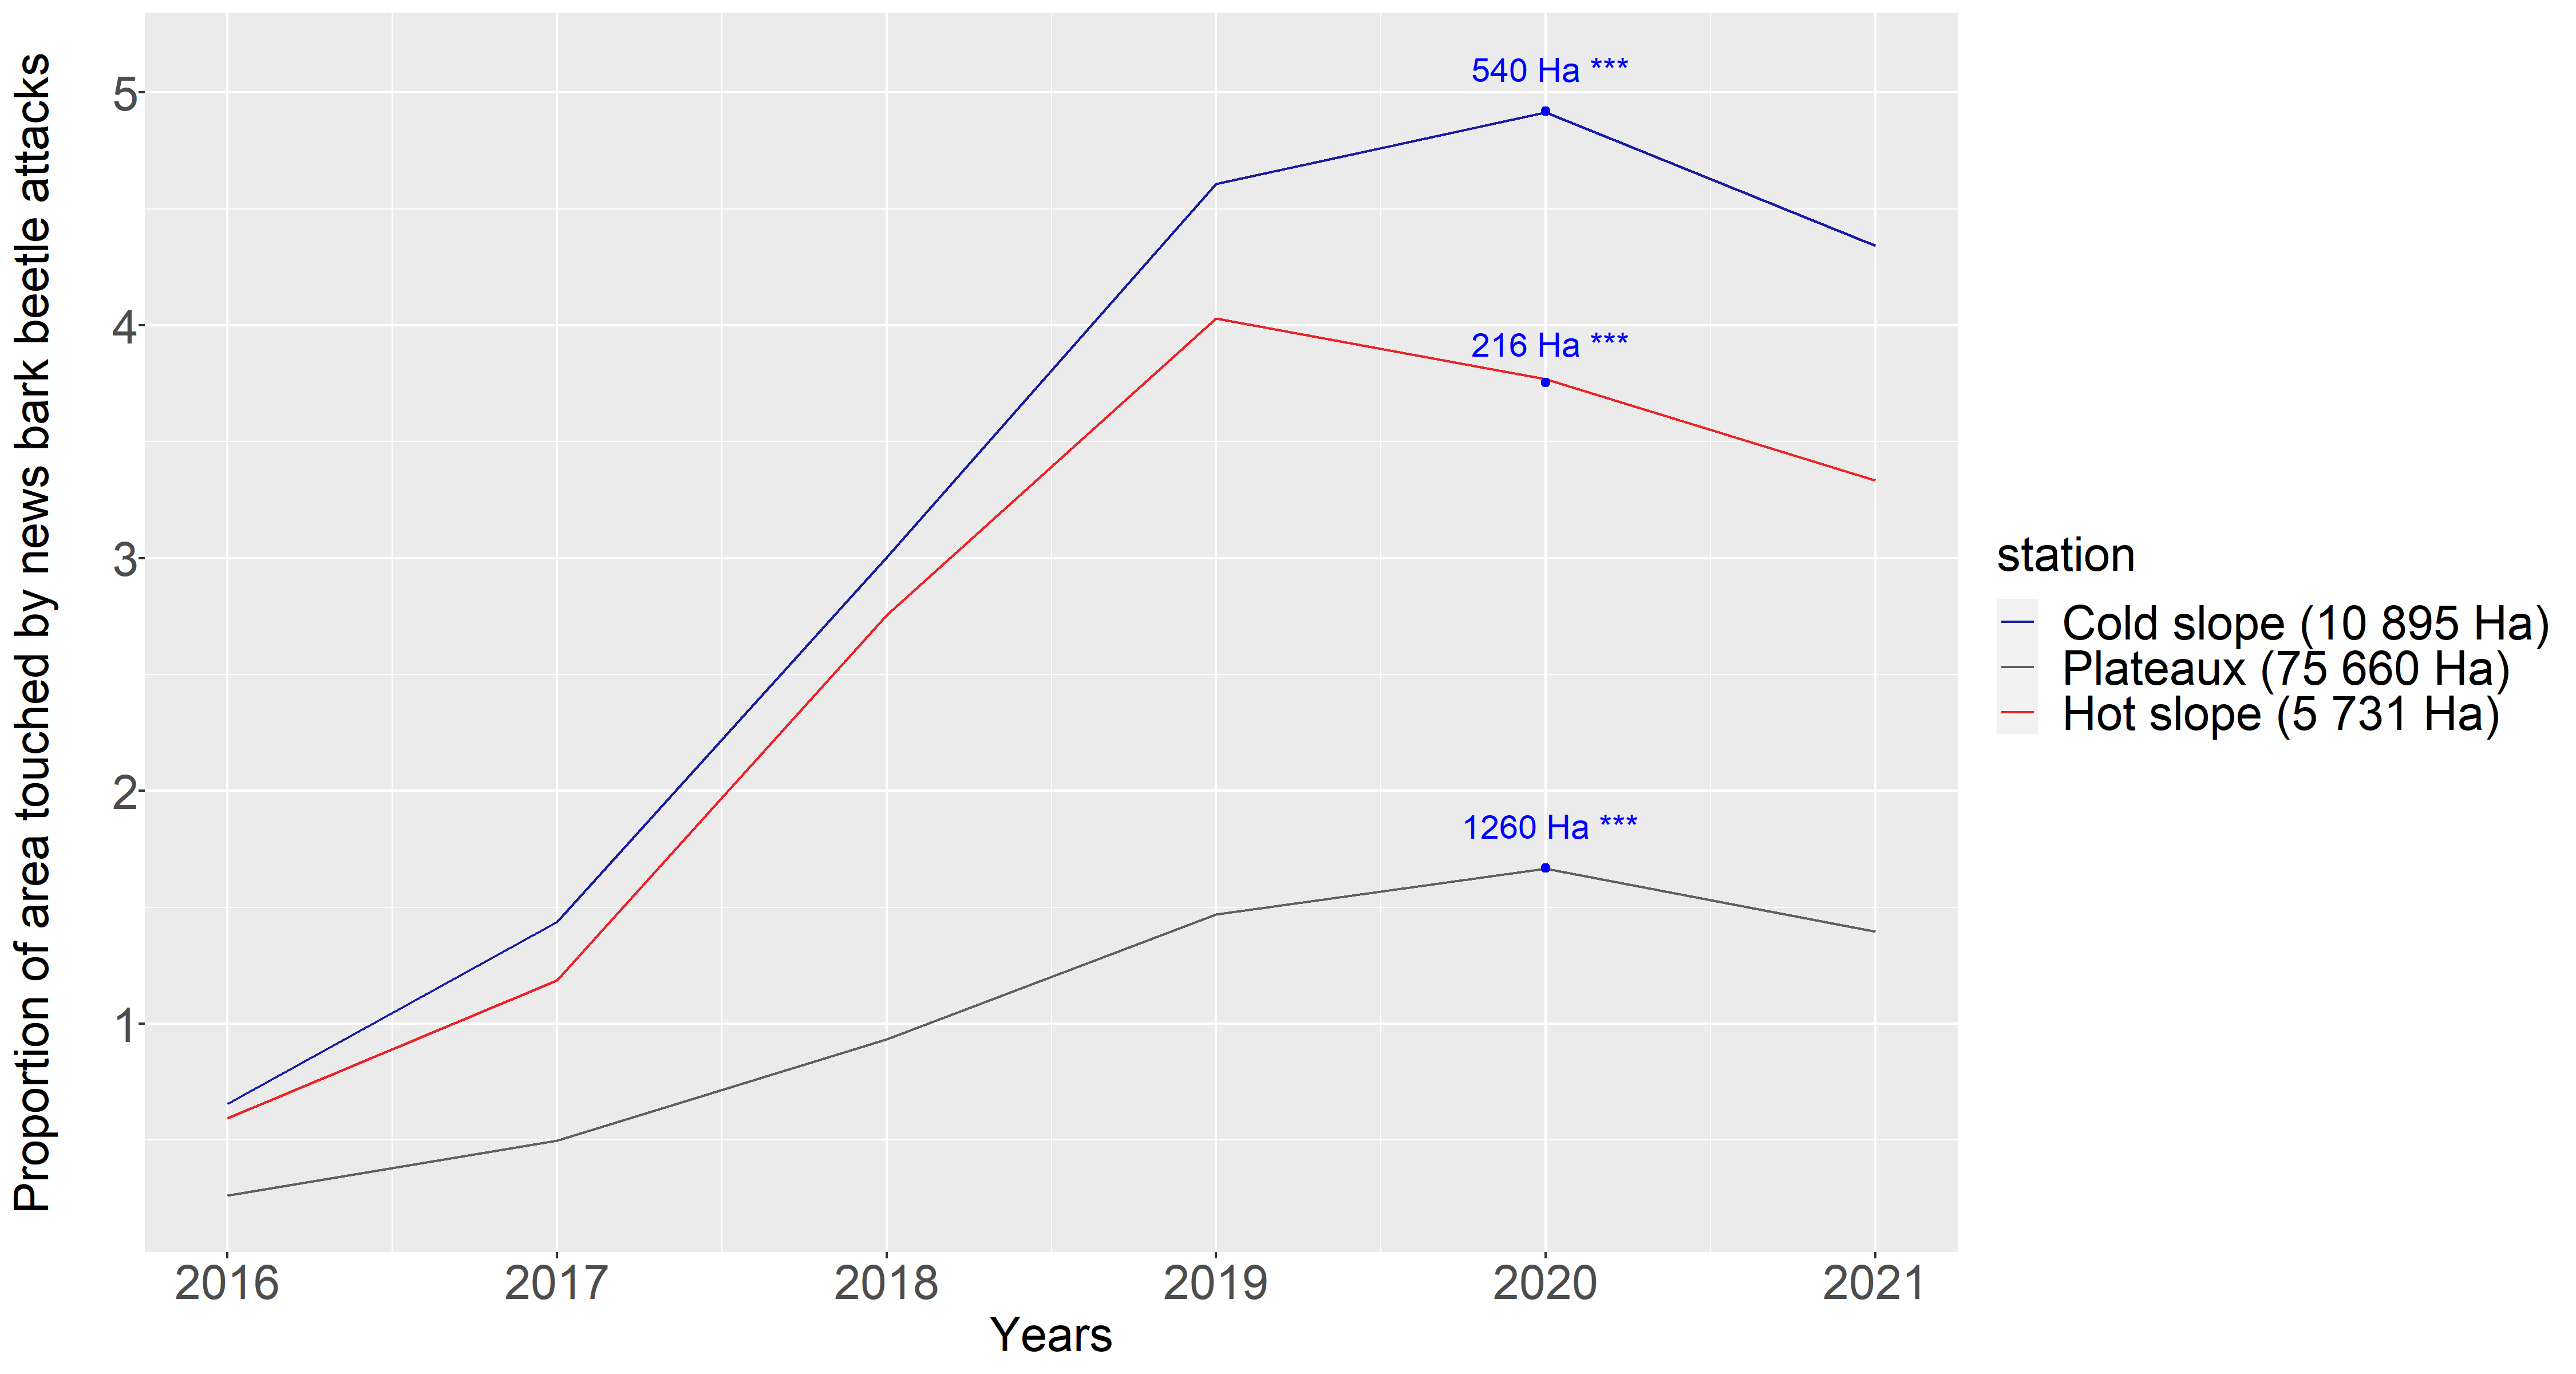
\includegraphics[width=1\textwidth]{evol_ss_wal.png}
		\caption{Évolution de la crise du typographe en région wallonne en fonction des sous-secteurs}
		\label{fig:topo}
		%\caption sert à insérer une légende
	\end{minipage}\hfill
	\vspace{0,5cm}
	\begin{minipage}[b]{1 \linewidth}
		\centering
		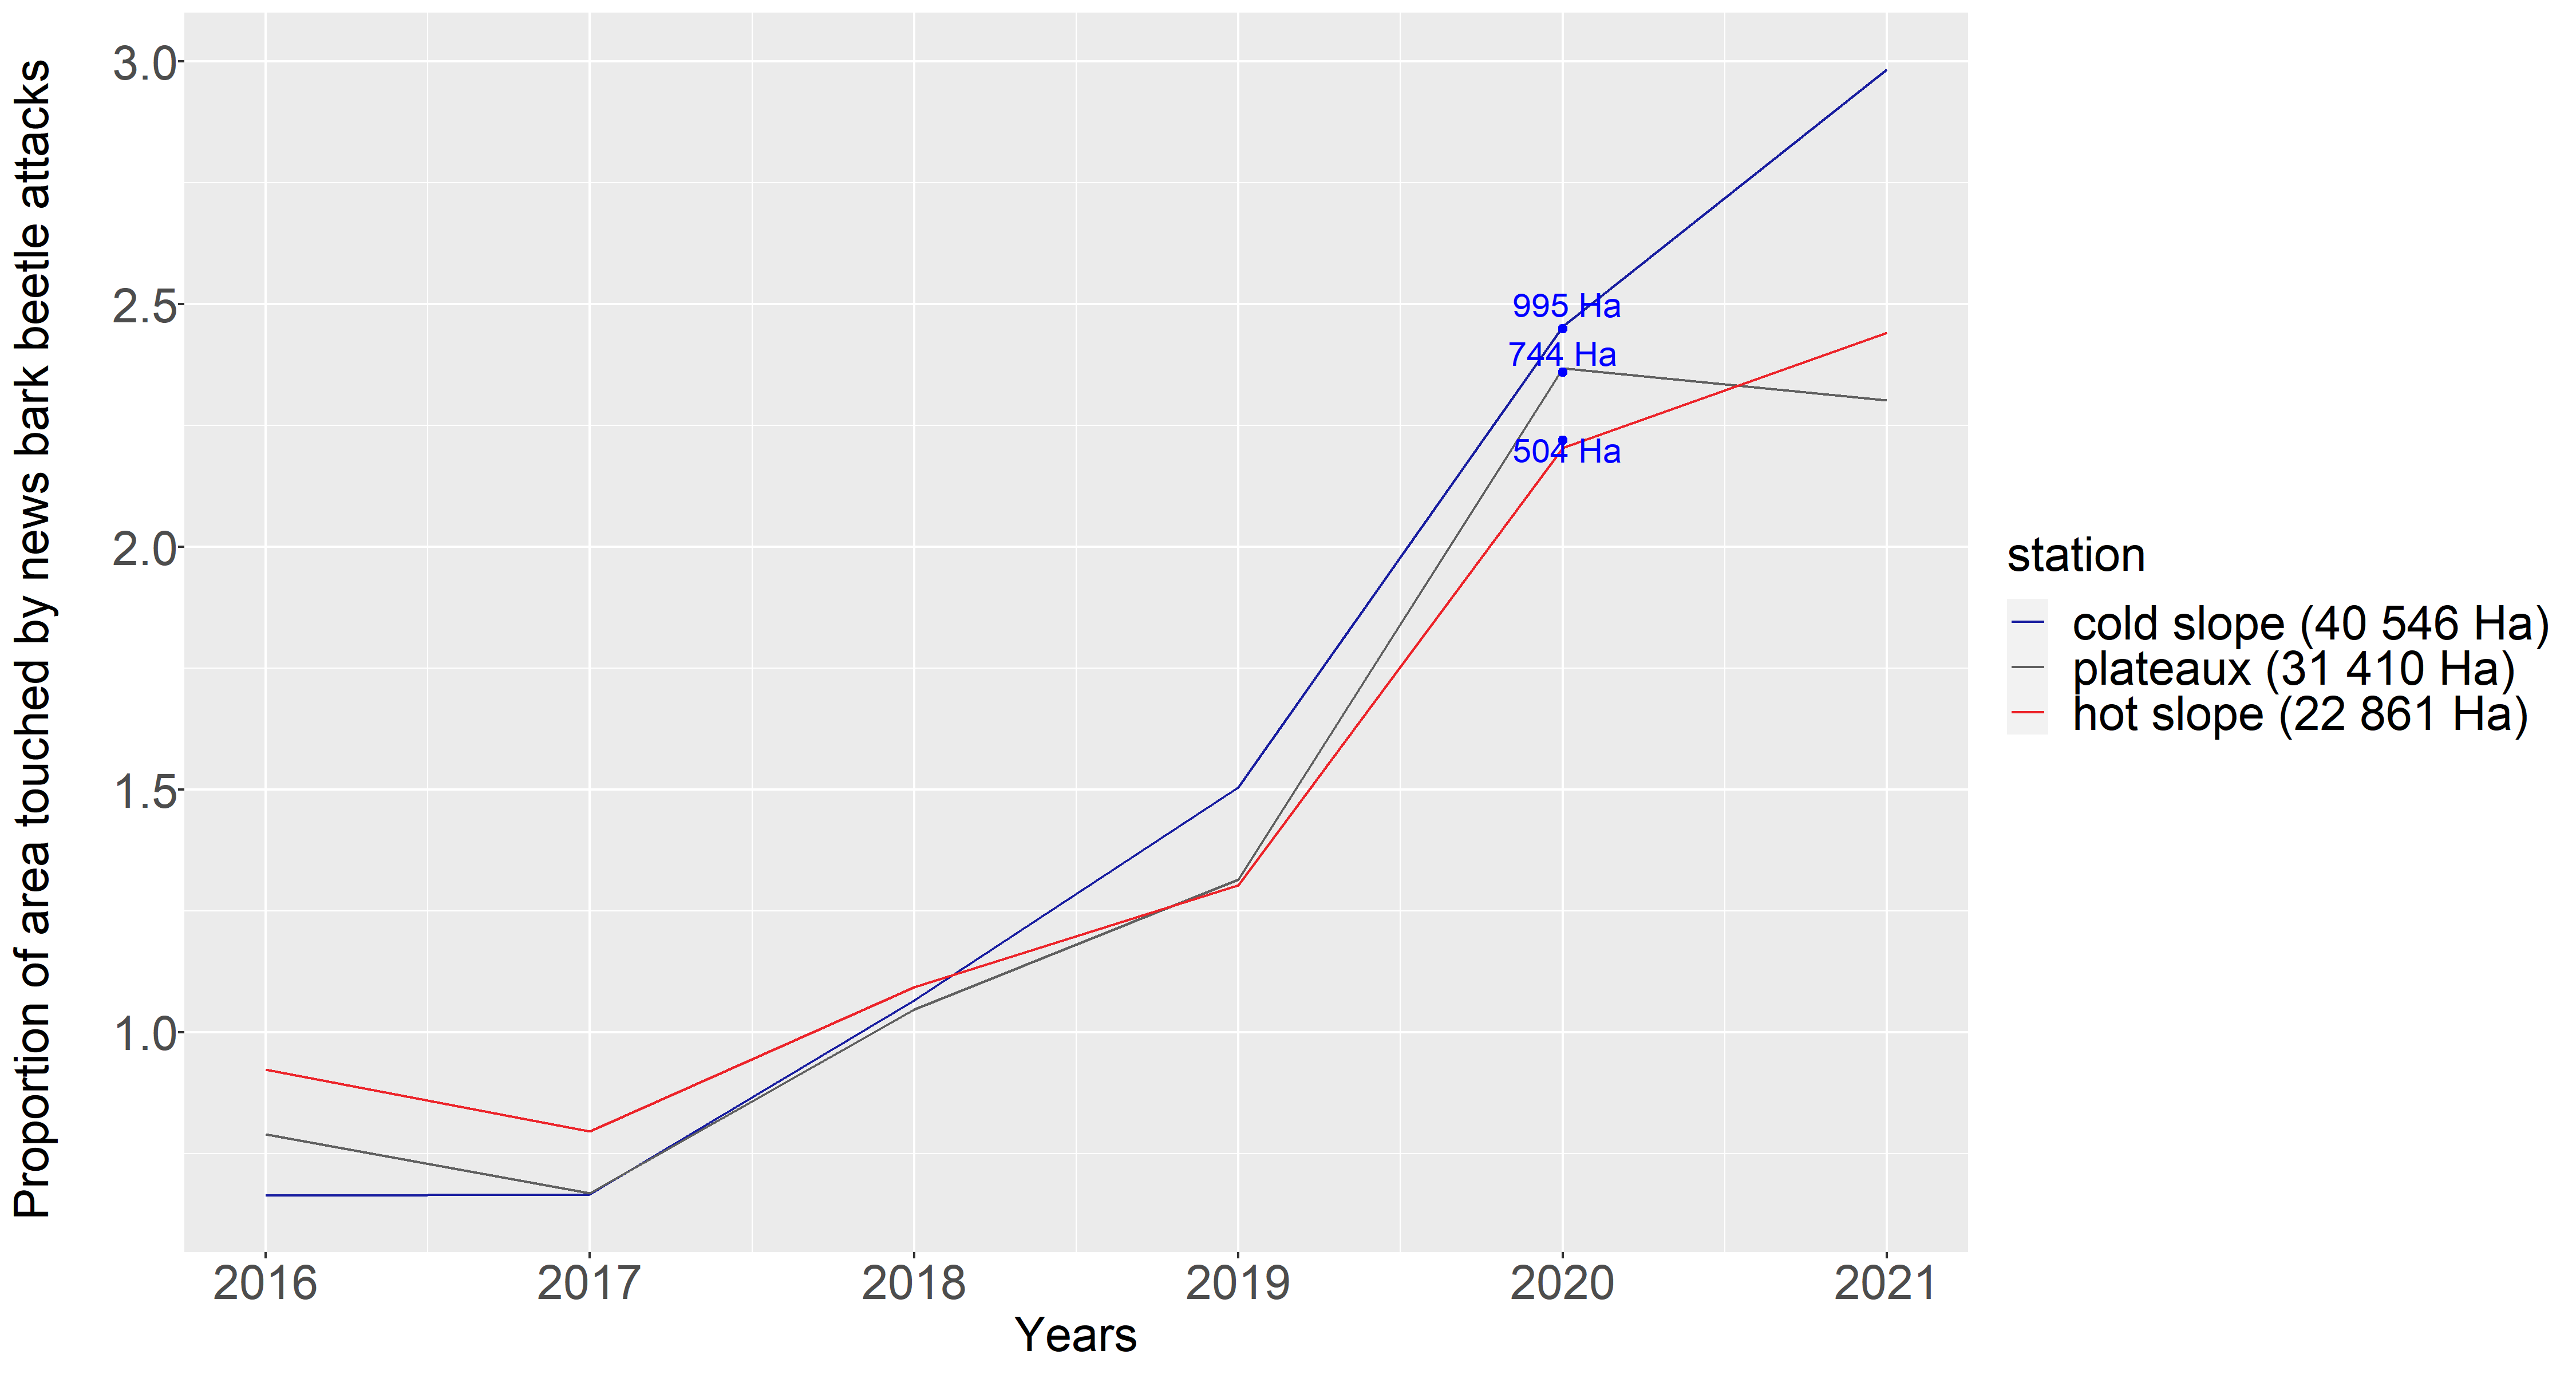
\includegraphics[width=1\textwidth]{evol_ss_vosges.png}
		\caption{Évolution de la crise du typographe dans les Vosges en fonction des sous-secteurs.}
		\label{fig:ss_vosges}
	\end{minipage}
\end{figure}




Ensuite, la probabilité de présence a été ventilée par année en fonction de chaque sous-secteur (figure \ref{fig:ss_vosges}). 
%Le code R employé est présent en Annexe. Le fichier d'input pour produire le raster Sous-secteur est le MNT.
%\begin{figure} [htbp] 
%  \centering
% 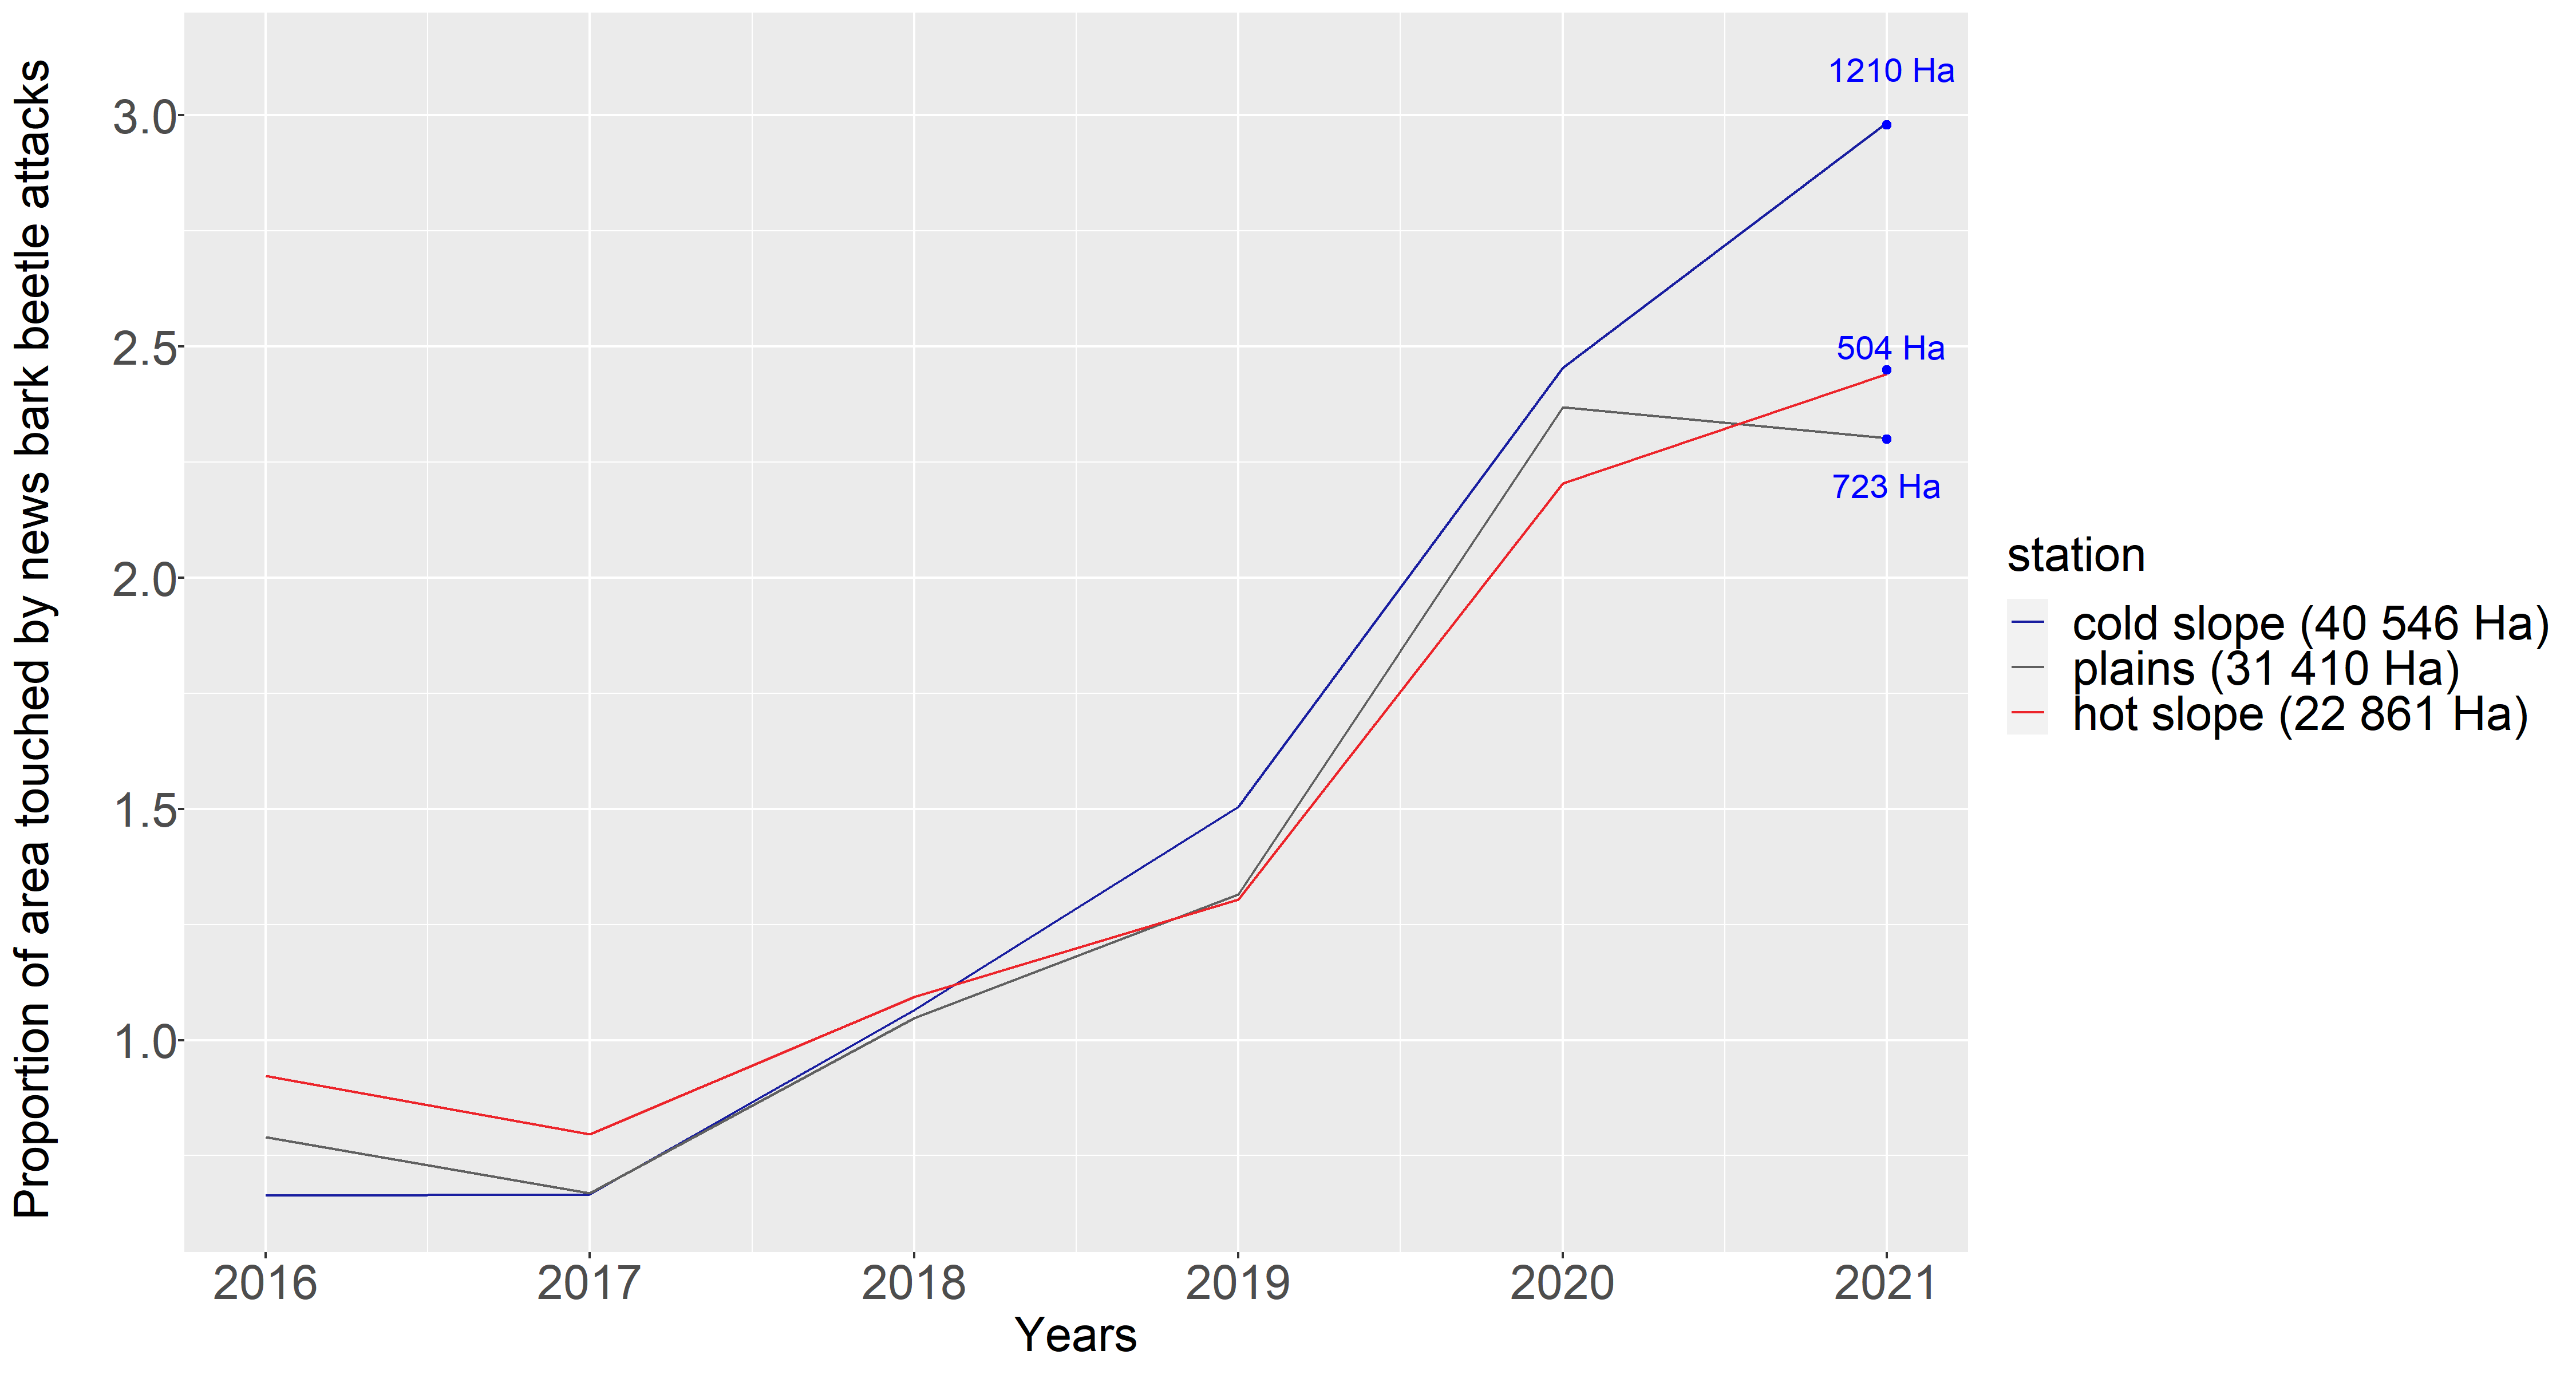
\includegraphics[width=1\textwidth]{evol_ss.png}
%\caption{Evolution de la crise du typographe dans les Vosges en fonction des sous-secteurs.}
%\label{fig:ss_vosges}
%\end{figure}

%definition sous secteur

Les probabilités de présence ont aussi été stratifiés en fonction du niveau d'altitude et des sous-secteurs.

%%description de la fih-gure des vosges
La figure \ref{fig:vosge} montre la variation de probabilité de présence de scolyte en fonction des sous-secteurs et par tranche d'altitude de 200 m dans les Vosges. Jusqu'en 2019, la probabilité de présence de scolyte est en augmentation continue.
%les sous secteur chaud semblent plus touchés sauf au delà de 800 m d'altitude et en dessous de 400 m d'altitude où les secteurs nord sont plus touchés. 
Cette probabilité de présence de scolyte reste inférieure à 5 pourcent quelque soit la tranche d'altitude et le sous-secteur.

Pour l'année 2020, il semble y avoir une augmentation de la probabilité de présence de scolyte. La probabilité de présence de scolyte dans les sous-secteurs neutres atteint les 10 pourcent dans les tranches d'altitude 200-400 m et 1000 à 1300 m. Dans les autres classes d'altitude, les sous-secteurs sont atteints de manière similaire.









\begin{figure} [htbp] 
	\centering
	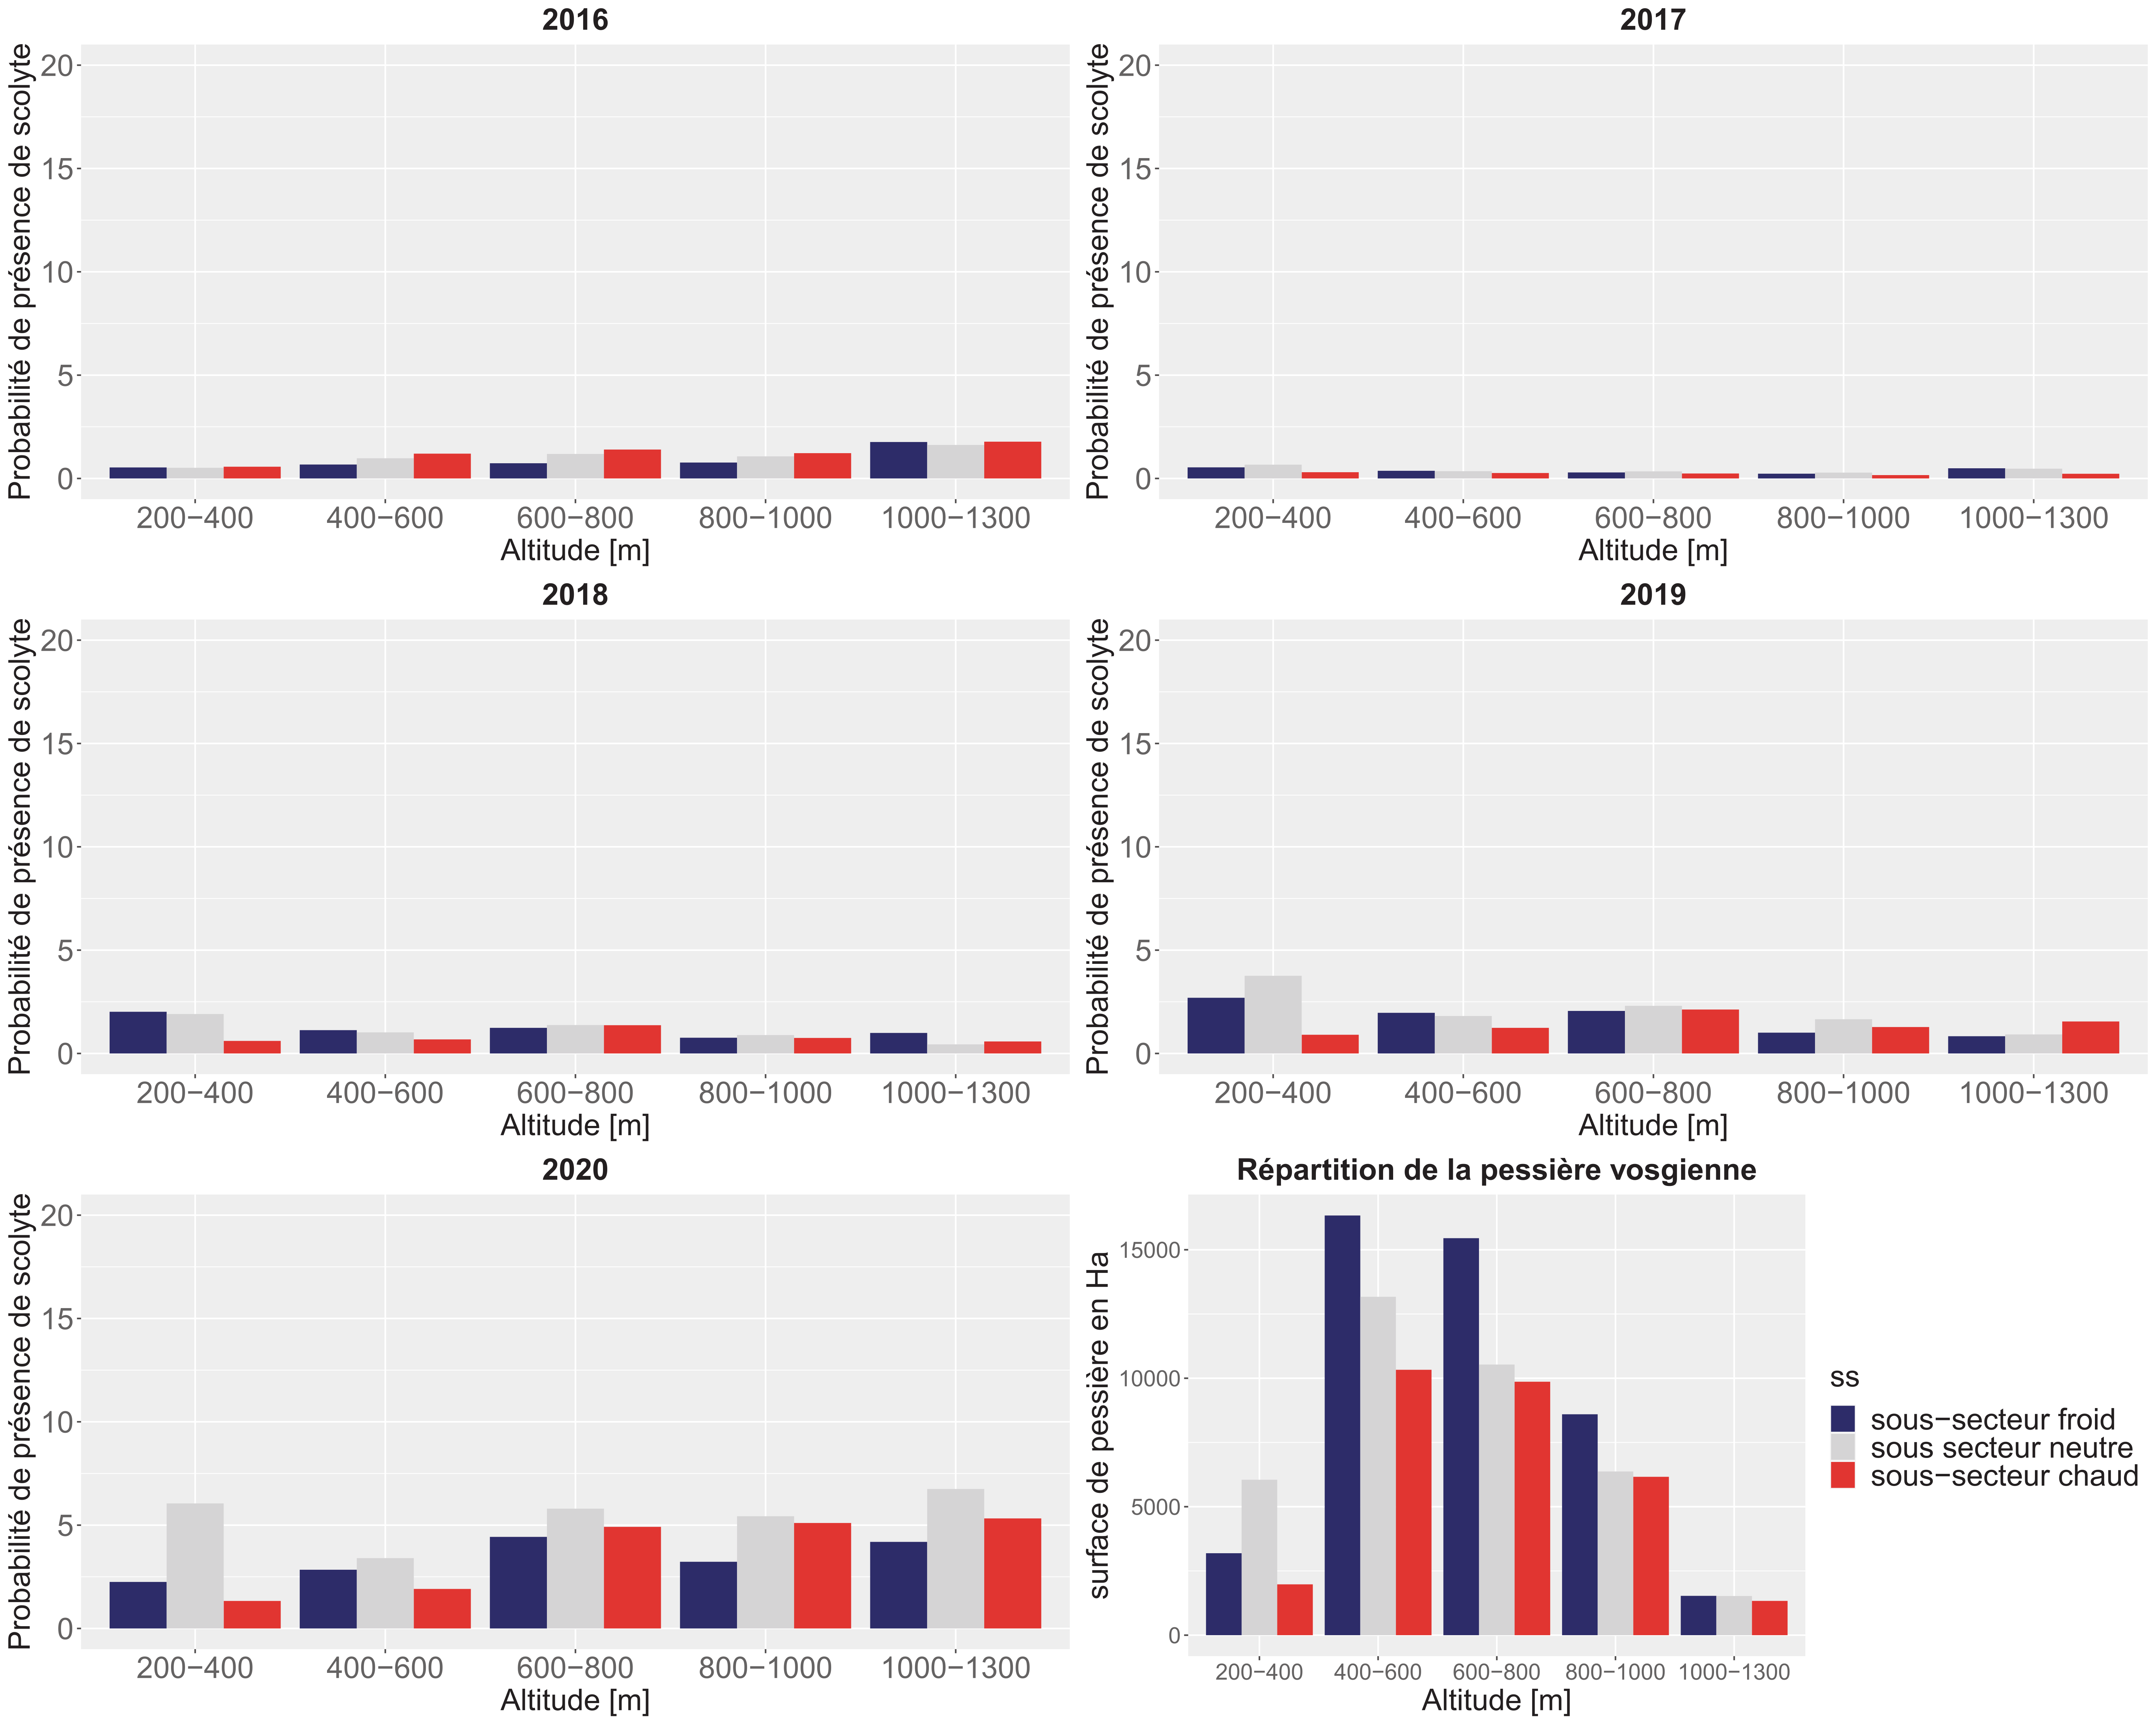
\includegraphics[width =1\textwidth]{alti_ss_vosges.png}
	\caption{Probabilité de présence de scolytes dans les Vosges entre 2016 et 2020 en fonction de l'altitude et des sous-secteurs}
	\label{fig:vosge}
\end{figure}

La figure \ref{fig:wall} montre que jusqu'en 2018 la probabilité de présence de scolyte dans les peuplements d'épicéas wallons est relativement faible quelque soit la classe d'altitude et le sous-secteur. Durant l'année 2018 la probabilité de présence de scolyte augmente dans les classes d'altitudes inférieures à 400 m tout en restant globalement inférieure à 5 \% de probabilité de présence de scolyte.
En 2019, la probabilité de présence de scolyte triple  dans la classe 100-200 m et double dans la classe 200-300 m. La classe 300-400 m est aussi touchée par une augmentation de la probabilité de présence mais moins intense que dans les deux classes d'altitudes inférieures. Dans les trois classes d'altitudes les plus faibles, les sous-secteurs chauds et froids semblent touchés de façon similaire et les secteurs neutres semblent moins impactés que les deux autres sous secteurs. \\

Concernant les classes d'altitude 100-200 m et 200-300 m, une augmentation de probabilité d'attaque dans les sous-secteurs neutres est à noter. 
Pour les classes d'altitude supérieure à 400 m, la probabilité de scolyte reste stable et inférieure à 5\%.
\begin{figure} [htbp] 
	\centering
	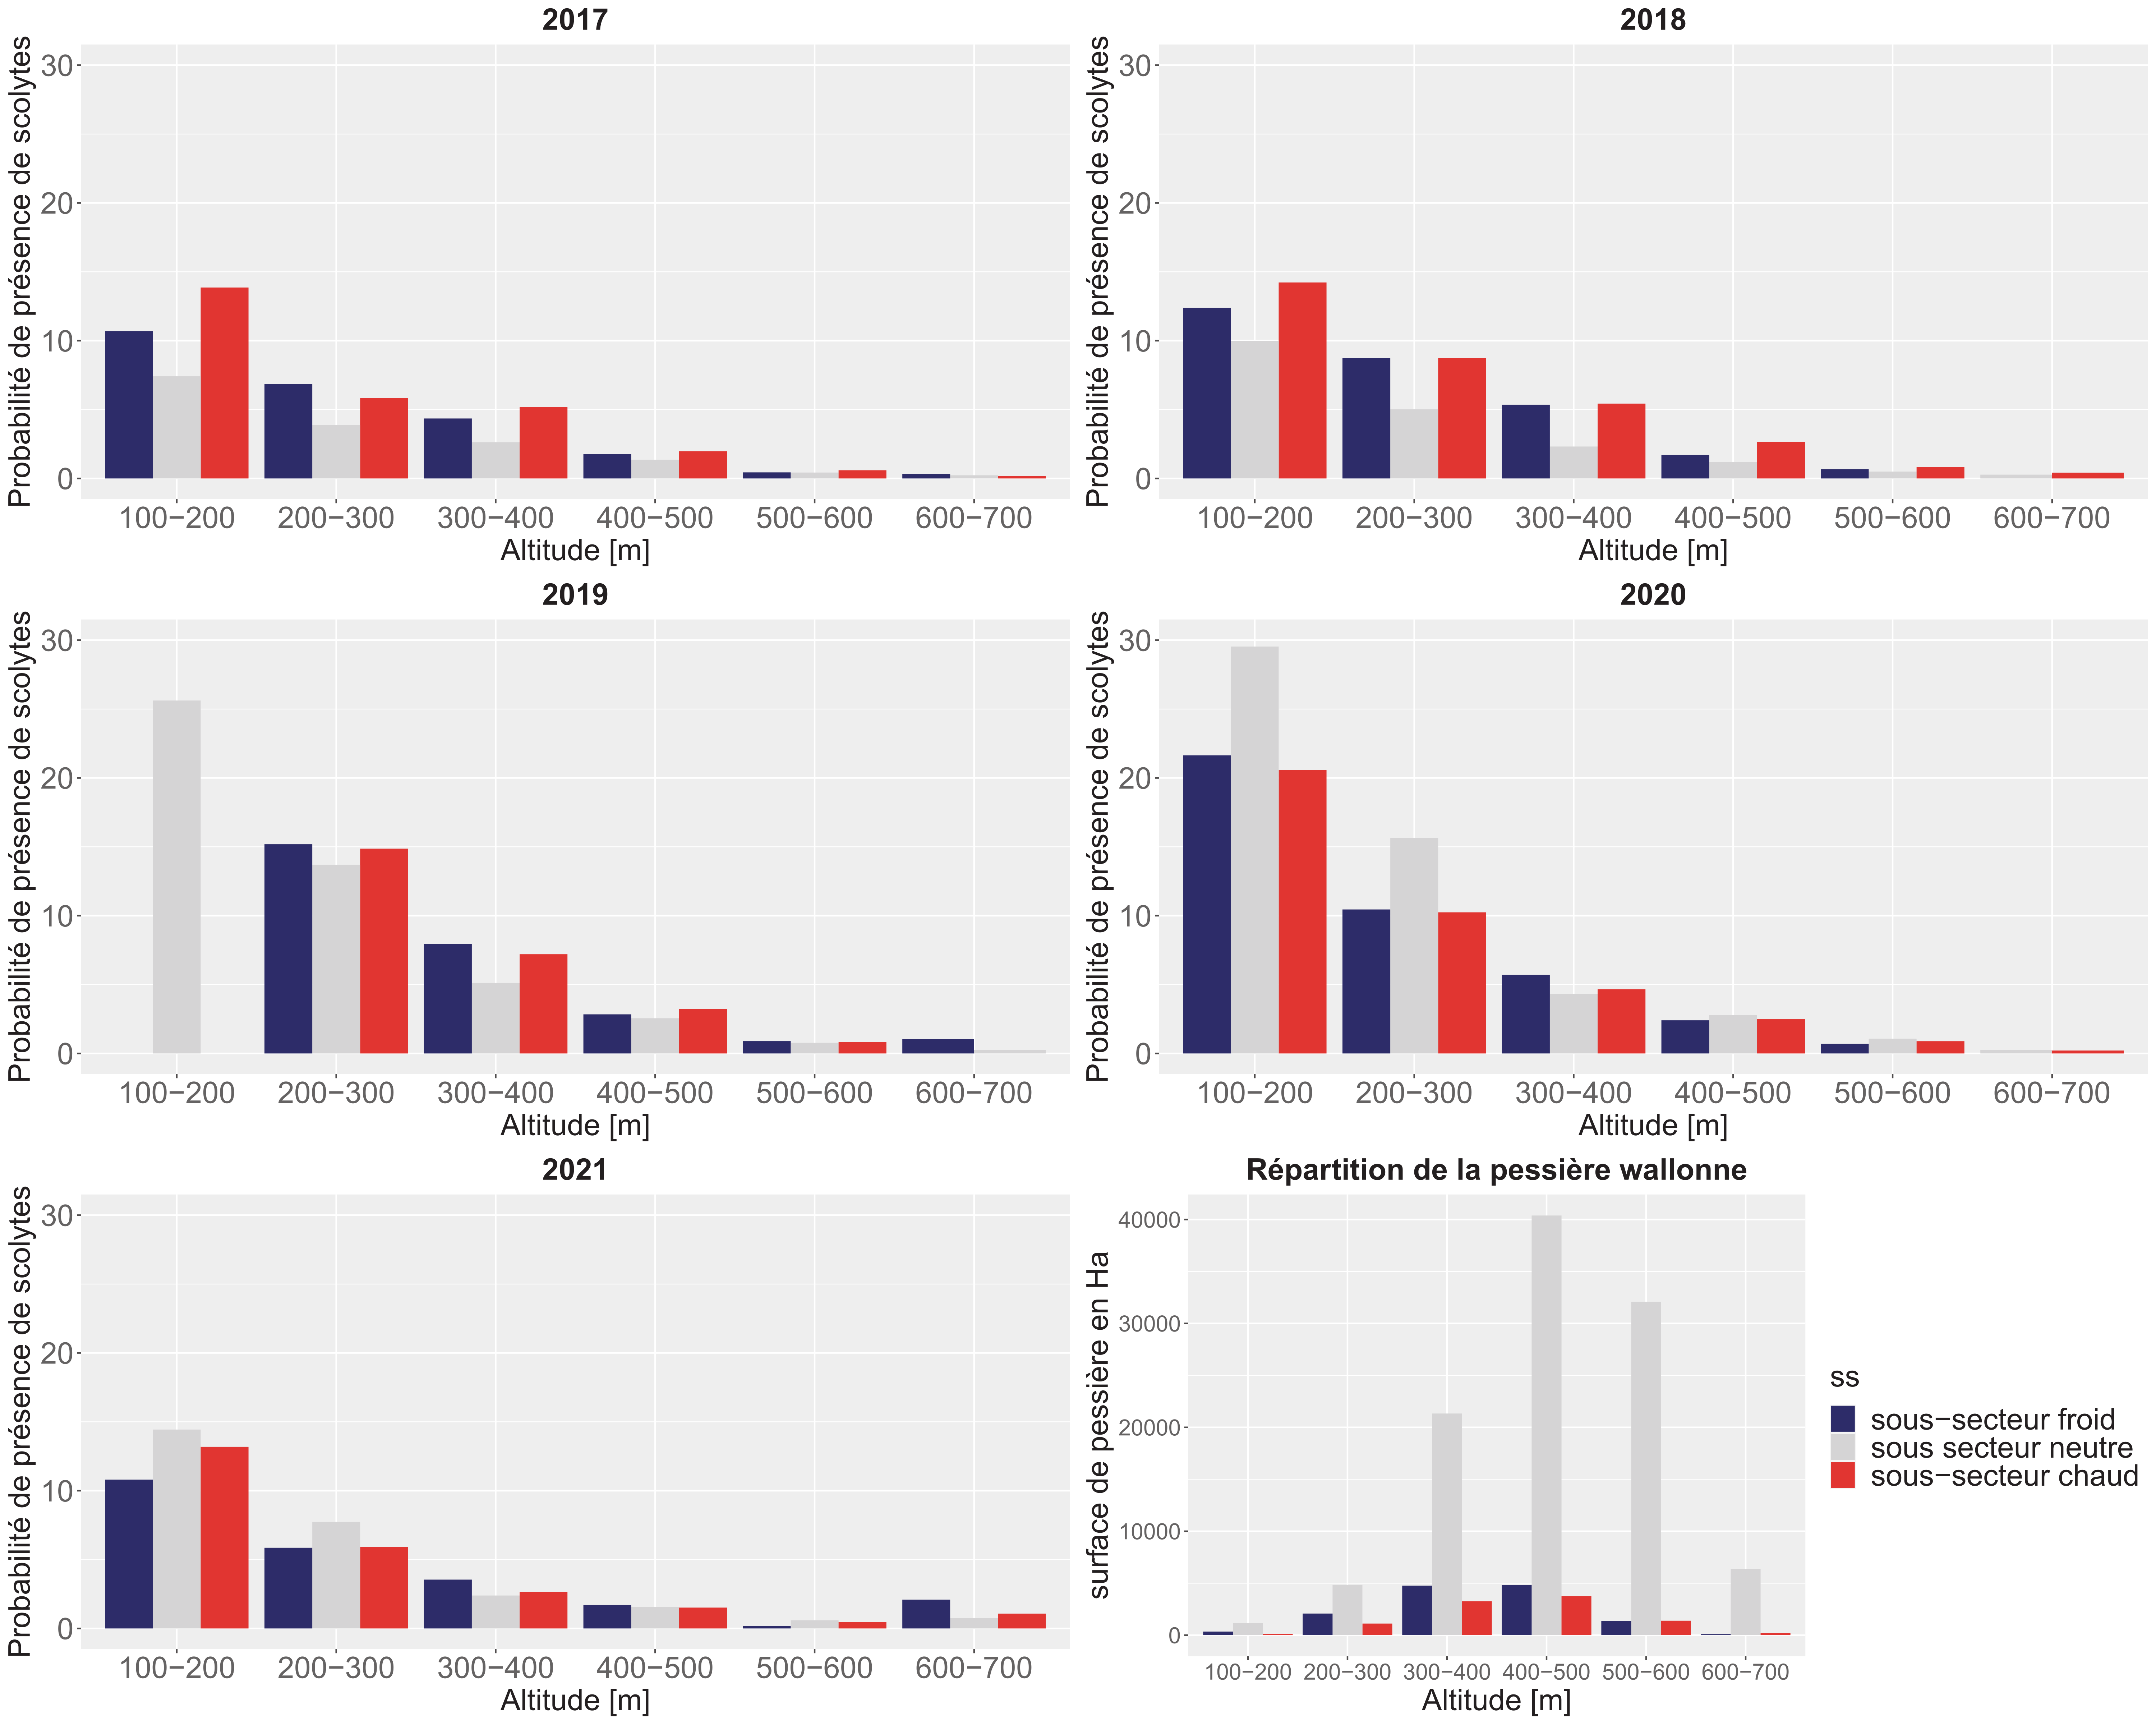
\includegraphics[width=1\textwidth]{alti_ss_wal.png}
	\caption{Probabilité de présence de scolytes en Wallonie entre 2016 et 2020 en fonction de l'altitude et des sous-secteurs }
	\label{fig:wall}
\end{figure}


 \section{Discussion}
\subsection{Comparaison des cartes de risque de BioClimSol et d'aptitude du Fichier Écologique}
A l'échelle régionale, le modèle BioClimSol et la carte d'aptitude du Fichier Écologique des Essences sont semblables. Cependant, à l'échelle locale, ces modèles diffèrent fortement.\\

L'origine de ces différences est probablement due aux hypothèses initiales des modèles:

\begin{itemize}
	\item le modèle BioClimSol est basé sur l'autécologie du scolyte. Pour ce modèle, la cause première du dépérissement des épicéas est l'attaque des scolytes qui pullulent grâce à des conditions météorologiques favorables;
	\item la carte d'aptitude du Fichier Écologique des Essences se base sur l'autécologie de l'épicéa. Ce modèle part de l'hypothèse que l'épicéa subit un stress suite à des conditions stationnelles qui ne lui sont pas propices. Le stress et l'affaiblissement permettent aux scolytes de le coloniser;
	\item le fichier écologique emploie des paramètres pédologiques (surtout pour le niveau hydrique);
\end{itemize}

Le modèle BioClimSol met plus en évidence un risque de scolyte qu'un risque autécologique, tandis que le Fichier Écologique des Essences montre plus un risque autécologique, même si le scolyte peut le révéler.






\subsection{Confrontation à l'aptitude}
Aucune des deux méthodologies ne permet de prédire le risque lié aux dégâts de scolyte. En effet, il n'existe aucune correspondance entre les aptitudes du Fichier Écologique ou  le niveau de risque de BioClimSol et les attaques de scolytes.

Le non fonctionnement des modèles peut être dû à l'extension des scolytes. En effet, la pullulation de cette insecte est plus ou moins indépendante de l'autécologie de l'épicéa. 
Par contre, si la pullulation des scolytes était liée à l'autécologie de l'épicéa, les modèles seraient à revoir ou à améliorer.

\subsection{Réponse des attaques de scolytes aux facteurs altitudinaux et topographiques.}

L'analyse des attaques de scolytes selon l'altitude et la position topographique , en Wallonie et dans les Vosges pose question.
\begin{itemize}
	\item en Ardenne, les attaques de scolytes sont plus marquées sur les versants, à l'inverse des prédictions du modèle BioClimSol, mais pas du tout dans les Vosges;
	
	\item l'effet micro-climatique de l'orientation des versants, attendu par le Fichier Écologique des Essences, ne se manifeste ni en Ardenne, ni dans les Vosges;
	
	\item les attaques de scolytes sont clairement inversement proportionnelles à l'altitude en Wallonie comme le niveau d'aptitude du Fichier Écologique des Essences pouvait le laisser présager, alors qu'elles ne sont étrangement pas influencées par ce facteur dans les Vosges.
	
\end{itemize}
On peut faire différentes hypothèses quant à la faible capacité de ces modèles à expliquer les attaques de scolytes:

\begin{itemize}
	\item l'explosion des populations de scolytes est indépendante des facteurs autécologiques de l'épicéa;
	\item les conditions météorologiques ont été trop différentes entre la zone ardennaise et vosgienne; les macro-climats ont peut-être des caractéristiques déterminantes différentes pour le scolyte ou l'épicéa (continentalité et caractère montagnard)
	\item Les paramètres de BioClimSol étant essentiellement liés au scolyte et ceux du Fichier Écologique des Essences essentiellement liés à l'épicéa, aucun de ces deux modèles ne peut rendre compte correctement du comportement du couple    scolyte/épicéa.
\end{itemize}

\newpage
\section{Conclusion}

Tant le modèle BioClimSol que celui du Fichier Ecologique des Essences sont peu efficaces pour prévoir les attaques de scolytes.

La comparaison des caractéristiques topographiques et altitudinales montre que les attaques de scolytes (typographes et chalcographes) sur les épicéas vosgiens et wallons sont différentes.\\

Toutefois, au niveau de la Wallonie, à une échelle macroscopique, l'échelle d'aptitude liée à l'altitude est en relation avec la probabilité de dégâts de scolytes ainsi que dans une moindre mesure , l'aptitude des zones biogéographiques.\\

BioClimSol, quant à lui, semble ne pas fonctionner à une échelle locale en Wallonie.






\bibliography{../../articleSco/Scolyte.bib}

\bibliographystyle{../s2_ts}

\end{document}
